 
 \documentclass[manuscript,screen=true, review, anonymous]{acmart}
 
 \usepackage[utf8]{inputenc}
 \usepackage{xspace}
 \usepackage{balance}
 \usepackage{amsmath,amsfonts,mathtools,amsthm}
 \usepackage{algorithmic}
 \usepackage{algorithm}
 
 \usepackage{balance}
 \usepackage[english]{babel}
 \usepackage{blindtext}
 \usepackage{amsthm,amsmath,array,colortbl,graphicx,multirow}
 \usepackage{comment}
 \usepackage{balance}
 \usepackage{tikz}
 \usepackage{amsmath}
 \usetikzlibrary{patterns} %
 \usepackage{algorithm}
 \usepackage[font={footnotesize}]{subcaption}
 \usepackage[font={footnotesize}]{caption}
 \usepackage{breakcites}
 \usepackage{booktabs}
 \usepackage{diagbox}
 \usepackage{xcolor}
 \usepackage{colortbl}
 \usepackage{cleveref}
 \usepackage{enumitem}
 
 \mathchardef\mhyphen="2D
 
 \title{Online Balanced Graph Partitioning: Optimizations for Large Clusters}
 
 \author{Maciej Pacut}
 \email{maciej.pacut@univie.ac.at}
 \orcid{0000-0002-6379-1490}
 \affiliation{%
 \institution{Faculty of Computer Science, University of Vienna}
 \country{Austria}
 }
 
 
 \author{Mahmoud Parham} 
 \email{mahmoud.parham@univie.ac.at}
 \orcid{0000-0002-6211-077X}
 \affiliation{%
 \institution{Faculty of Computer Science, University of Vienna}
 \country{Austria}
 }
 
 \author{Stefan Schmid} 
 \email{stefan_schmid@univie.ac.at}
 \affiliation{%
 \institution{Faculty of Computer Science, University of Vienna}
 \country{Austria}
 }
 
 \copyrightyear{2020} 
 \acmYear{2020} 
 \setcopyright{acmlicensed}
 \acmConference{DISC '20}{October 12-16, 2020}{Freiburg, Germany}
 
 \keywords{online algorithms, competitive analysis, graph partitioning, clustering}
 \acmISBN{}\acmPrice{}
 \acmDOI{}
 
 \ccsdesc[500]{Networks~Network algorithms}
 \ccsdesc[300]{Computer systems organization~Cloud computing}
 \ccsdesc[300]{Computer systems organization~Distributed architectures}
 
 %%%%%%%%%%%%%%%%%%%%%%%%%%%%%%%%%%%%%%%%%%%%%%%%&&
 %%%%%%%%%%%%%%%%%%%%%%%%%%%%%%%%%%%%%%%%%%%%%%%%&&
 %  our macros start
 %%%%%%%%%%%%%%%%%%%%%%%%%%%%%%%%%%%%%%%%%%%%%%%%&&
 %%%%%%%%%%%%%%%%%%%%%%%%%%%%%%%%%%%%%%%%%%%%%%%%&&
 
 \newcommand{\OPT}{\textsf{OPT}\xspace}
  \newcommand{\OPTM}{\mathit{OPT}}
 \newcommand{\ALG}{\textsf{ALG}\xspace}
 \newcommand{\PPL}{\textsf{PPL}\xspace}
 \newcommand{\OBRP}{BRP}
 \newcommand{\PPOBRP}{PP-BRP}
 \newcommand{\dist}{\textsf{dist}}
 \newcommand{\TAlg}{{\ensuremath{\textsf{ALG}_{3}}}\xspace}
  \newcommand{\RM}{\textsf{RM}\xspace} % rematching alg
 
 \newcommand{\comm}{\textsc{comm}}
 \newcommand{\OFF}{\textsc{Off}\xspace}
 \newcommand{\Rep}{\textsc{Rep}}
 
 
 
 
 \newtheorem{claim}{Claim}
 \newtheorem{fact}{Fact}
 \newtheorem{rem}{Remark}
 \newtheorem{observation}{Observation}
 \newtheorem{property}{Property}
 
 
 \DeclarePairedDelimiter\pair{(}{)}
 \DeclarePairedDelimiter\set{\{}{\}}
 
 \DeclarePairedDelimiter{\ceil}{\lceil}{\rceil}
 \DeclarePairedDelimiter{\floor}{\lfloor}{\rfloor}
 
 \newcommand\mahmoud[1]{\color{orange}\textbf{Mahmoud: #1~}\color{black}}
 \newcommand\stefan[1]{\color{blue}\textbf{Stefan: #1}\color{black}}
 \newcommand\maciek[1]{\color{brown}\textbf{(Maciek: #1)}\color{black}}
 %\newcommand\mahmoud[1]{}
 %\newcommand\stefan[1]{}
 %\newcommand\maciek[1]{}
 
 
 \newcommand{\todo}[1]{\noindent\color{brown}{todo: #1}\color{black}}
 
 \begin{CCSXML}
	<ccs2012>
	<concept>
	<concept_id>10003033.10003068</concept_id>
	<concept_desc>Networks~Network algorithms</concept_desc>
	<concept_significance>500</concept_significance>
	</concept>
	<concept>
	<concept_id>10010520.10010521.10010537.10003100</concept_id>
	<concept_desc>Computer systems organization~Cloud computing</concept_desc>
	<concept_significance>300</concept_significance>
	</concept>
	<concept>
	<concept_id>10010520.10010521.10010537</concept_id>
	<concept_desc>Computer systems organization~Distributed architectures</concept_desc>
	<concept_significance>300</concept_significance>
	</concept>
	</ccs2012>
\end{CCSXML}

% for my small screen
%\setlength{\textwidth}{8cm}

\begin{document}

\begin{abstract}
	Distributed   applications,  including  batch  processing, streaming, scale-out databases,
	or machine learning, generate a significant amount of network traffic. By collocating frequently communicating nodes (e.g., virtual machines) on the same clusters (e.g., server or rack), the network load can be reduced and application performance improved. 
	However, as the communication pattern is a priori unknown and may change over time, it needs to be learned efficiently, in an online manner.
	%
	This paper revisits the online 
	balanced repartitioning problem 
	(introduced by Avin et al.~at DISC 2016)
	which asks for an algorithm that strikes
	an optimal tradeoff between the benefits
	of collocation (i.e., lower network load) 
	and its costs (i.e., migrations). 
	%
	Our first contribution is a significantly improved
	lower bound of $\Omega(k\cdot \ell)$ on the
	competitive ratio, where $\ell$ is the number
	of clusters and $k$ is the cluster size,
	even for a scenario in which the communication
	pattern is static and can be perfectly partitioned;
	we also provide a tight upper bound 
	of $O(k\cdot \ell)$ for this scenario.
	In addition, we present a tight upper bound
	of $\Theta(\ell)$ for $k=3$,
	for the general model in which the
	communication pattern can change arbitrarily
	over time. 
\end{abstract}

\maketitle

\renewcommand{\shortauthors}{M.~Pacut, M.~Parham, S.~Schmid}

\maciek{TODOs: "requests between nodes" to "requests to pair of nodes"}

\section{Introduction}

\maciek{Practical motivation}

\subsection{Model.}

\maciek{We study two models. One is a subproblem.}

The general model, where $\sigma$ can be arbitrary
was the original problem introduced
by Avin et al.~\cite{repartition-disc} at DISC 2016.
For simplicity, we will refer to the Perfect Partition
model as the \emph{learning} model (as
one has to learn the static communication graph) 
and to the original as the \emph{repartitioning} model (as one continuously adjusts the partition in response to changing communication graph).

\subsubsection{Partitioning model.}
The \emph{balanced repartitioning} problem (\OBRP{})
is a fundamental learning problem
that finds applications in the context of
distributed systems optimization~\cite{repartition-disc}. We are given a set $V$ of $n$ nodes 
(e.g., virtual machines or processes),
initially arbitrarily partitioned into $\ell$~clusters
(e.g., servers or entire racks),
each of size~$k$.
The nodes interact using
a sequence of pairwise communication requests
$\sigma = (u_1,v_1),$ $(u_2,v_2),$ $(u_3,v_3), \ldots$,
where a pair $(u_t,v_t)$ indicates that nodes $u_t$ and $v_t$ exchange a~certain amount of data.
Nodes in $C \subset V$ are \emph{collocated}
if they reside in the same cluster.

An algorithm serves a communication request between two nodes
either \emph{locally} at cost~0
if they are collocated,
or \emph{remotely} at cost~1
if they are located in different clusters.
We refer to these two types of requests as \emph{internal}
and \emph{external} requests, respectively.
Before serving a request,
an online algorithm may perform a \emph{repartition},
%(i.e., \emph{reconfigure}).
i.e.,
it may move (``migrate'') some nodes into clusters different from their current clusters, while respecting the capacity of every cluster. 
Afterwards, 
the algorithm serves the  request.
The cost of migrating a node from one cluster to another
is~$\alpha \in \mathbb{Z}^+$.
\maciek{Why restrict $\alpha$? It should just be positive}
For any algorithm $\ALG$,
its cost,
denoted by $\ALG(\sigma)$,
is the total cost of communications and
the cost of migrations performed by $\ALG$ while serving the sequence $\sigma$.

\maciek{The competitive ratio definition and the worst case inputs}

\maciek{Ilustrate the challenges. Rent-or-buy. Decision what to evict}


\subsubsection{Learning model.}
In addition to the general model, we study a simplified Perfect Partition model (also studied by Henzinger et al.~\cite{sigmetrics19_partitioning} (SIGMETRICS 2019)) that we consider for a stronger lower bound.
There, we assume that $\sigma$
reveals the edges of a static graph
that can be perfectly partitioned
(no external requests are required). 



\subsection{Related work}


The existing results in~\cite{repartition-disc} and~\cite{sigmetrics19_partitioning} primarily focus on a model with resource augmentation, where  the online algorithm has slightly larger clusters than the offline algorithm.
They showed that their lower bound $\Omega(k)$ holds even for a significant resource augmentation.
They provided an algorithm with the competitive ratio independent of $\ell$ using the $(2+\epsilon)$-augmented cluster capacity.


In contrast, we study the non-augmented setting, where the nodes need to be perfectly balanced  among the clusters.
In the paper that originated a study on BRP \cite{repartition-disc} (DISC 2016), authors provided a $O(k^2 \cdot \ell^2)$-competitive algorithm, and a lower bound $\Omega(k)$.
For $k=2$, they presented a $7$-competitive algorithm~\cite{repartition-disc} with a~substantial ($\Omega(\ell^2)$) additive constant.


The problem has also been studied in a weaker
model where the adversary can only sample
requests from a fixed distribution~\cite{stochastic-ring}.



\maciek{Offline results}
\maciek{Links other problems: for $k=2$ a flavor of online matching, for $\ell = 2$ it generalizes paging}

%More generally, the model is related to online
%caching~\cite{SleTar85,FKLMSY91,McGSle91,AcChNo00},
%see~\cite{repartition-disc} for a discussion.
%The static offline version of~the~problem, called the
%\emph{$\ell$-balanced graph partitioning problem} is 
%NP-complete, and cannot even be approximated within %any finite factor unless P
%= NP~\cite{AndRae06}. 

\subsection{Our Contributions.}
We provide an improved lower bound 
of $\Omega(k\cdot\ell)$ on the competitive ratio of any online deterministic online algorithm 
even in the learning model;
the best known lower bound so far was $\Omega(k)$,
even for a more general model~\cite{repartition-disc}.
We also present an asymptotically optimal, 
$O(k\cdot \ell)$-competitive algorithm
for the learning model.
For the repartitioning model, we present  
an asymptotically optimal,
$\Theta(\ell)$ algorithm for $k=3$;
the best known upper bound 
so far was $O(\ell^2)$~\cite{repartition-disc}.
Then, we present a strictly $6$-competitive algorithm for $k=2$ that improves upon previous $7$-competitive algorithm with $O(\ell^2)$ additive constant..
In addition, we show a new, improved analysis of the algorithm from \cite{repartition-disc} that depends on the solutions to an interesting combinatorial problem (see Section~\ref{ssec:cascade}, The Cascade Problem).
%
The overview of known results is in Table~\ref{tab:overview}.

\begin{table*}
	\centering
	\renewcommand{\arraystretch}{1.5}
	\begin{tabular}{>{\centering\arraybackslash}p{4.5cm}|>{\centering\arraybackslash}p{4.5cm}>{\centering\arraybackslash}p{4.5cm}}
		\rowcolor{gray!50}
		\textbf{Variant} & \textbf{ Lower bound} &\textbf{Upper bound}\\ \hline 
		\textbf{$k=2$}& 3\hspace{0.3cm}\cite{repartition-disc} & 6\hspace{0.3cm}(\S \ref{sec:k2}) \\ 
		\rowcolor{gray!25}
		\textbf{$k=3$}&  $\Omega(\ell)$ \hspace{0.3cm}(\S \ref{sec:lowerbound})& $O(\ell) $\hspace{0.3cm}(\S \ref{sec:k3})\\
		$k > 3$ & $\Omega(k\cdot \ell)$\hspace{0.3cm}(\S  \ref{sec:lowerbound})&$O(k \cdot \ell \cdot \min \{ k \cdot \ell, \Rep(k, \ell) \})$\hspace{0.1cm} (\S \ref{sec:k3}) \\
		\rowcolor{gray!25}
		Learning model & $\Omega(k\cdot \ell)$\hspace{0.3cm}(\S  \ref{sec:lowerbound})&$O(k \cdot \ell)$\hspace{0.3cm} (\S \ref{sec:ppl}) \\
	\end{tabular}
	\caption{Overview of known results and the results provided in this paper. By $\Rep$ we denote the cost of a single component repartition, and we elaborate on this in Section~\ref{sec:k3}. The results pertain to the general partitioning model, but the last row, that pertains to the learning model for arbitrary $k$ and $\ell$.
	}
	\label{tab:overview}
	\vspace{-7mm}
\end{table*}

\section{Preliminaries.}
\label{sec:prelim}

Across this paper, we often refer to groups of communicating nodes.
We use this concept slightly differently in the lower bound and the upper bounds.
In our algorithms, we group nodes with a communication history into \emph{components}, and in the lower bound, we group nodes that may communicate into \emph{ground sets}.

\noindent
\textbf{Components.}
In our algorithms, a~\emph{component} is a subset of frequently communicating nodes.
We maintain all nodes of each component collocated in one cluster~\cite{repartition-disc}.
If we need to move a node, we move the whole component that contains it.
We maintain a balanced partition of our components, a similar concept to partition of integers into sets with equal sum (\maciek{TODO: cite}).
In contrast, our partition is time-varying: communicating components are merged into one, and we adjust the partition.

\noindent
\textbf{Ground sets.}
In the lower bound, a~\emph{ground set} is a group of nodes that repeatedly communicate when an algorithm splits them (places at different clusters).
Their role is to ensure that the algorithm maintains a partition of ground sets into clusters.
We emphasize that ground sets are revealed only upon their nodes are split.
%\maciek{Other names: division, segmentation, alignment, formation}

%We say that the request $(u,v)$ is \emph{external}, if the algorithm is in the configuration, where $u$ and $v$ are located at different clusters.
%This is achieved by opting a sequence of  partitions (a.k.a.~configurations)
%such that frequently communicating nodes (from different clusters)
%are relocated to the same cluster before they inflict too much communication cost.
%A \emph{reconfiguration} (i.e.,\emph{ re-partitioning})
%is performed by migrating nodes between clusters,
%at the total cost of individual node migrations.
%The objective is to jointly minimize communication and migration costs while serving the sequence.

We say that a component or a ground set is \emph{trivial}, if it contains exactly one node.
We say that the node that belongs to trivial component or a ground set is \emph{alone}.
We say that a~configuration is \emph{component-respecting}
if the nodes belonging to the same component are collocated.



\section{The Learning Problem} %$\Omega(k\cdot \ell)$ for Competitive Ratio of Any Deterministic Algorithm}

In this section we consider a variant of Online Balanced Partitioning, where communication requests are permanent: once a pair of nodes start communicating, they continue forever.
To avoid infinite cost, each communicating pair must be collocated.
We study instances with finite cost: we assume that the communication graph can be perfectly partitioned in the clusters.
The algorithm's goal is to \emph{learn} the communication graph, and partition it without too many reconfigurations.


For this setting, we show a surprisingly high lower bound of $\Omega(k \cdot \ell)$.
The lower bound can be easily translated to the partitioning model (studied in Section~\ref{sec:part}) with finite request sequence.
At the end of this section, we discuss an asymptotically optimal upper bound.


\subsection{Lower bound.}

\label{sec:lowerbound}


We provide a lower bound $\Omega(k\cdot \ell)$ for the competitive ratio of any deterministic online algorithm for the learning problem.
Later we elaborate on how to efficiently transform it to a lower bound for the partitioning problem.
The lower bound requires $k\geq 3$.
For $k=2$, the learning problem is trivial: immediate collocation of a communicating pair is $1$-competitive.
(A partitioning problem for $k=2$ is non-trivial, a lower bound of $3$ is known \cite{repartition-disc}, and we provide a $6$-competitive algorithm (see Section~\ref{sec:k2}).)




\begin{figure}[H]
	\centering
	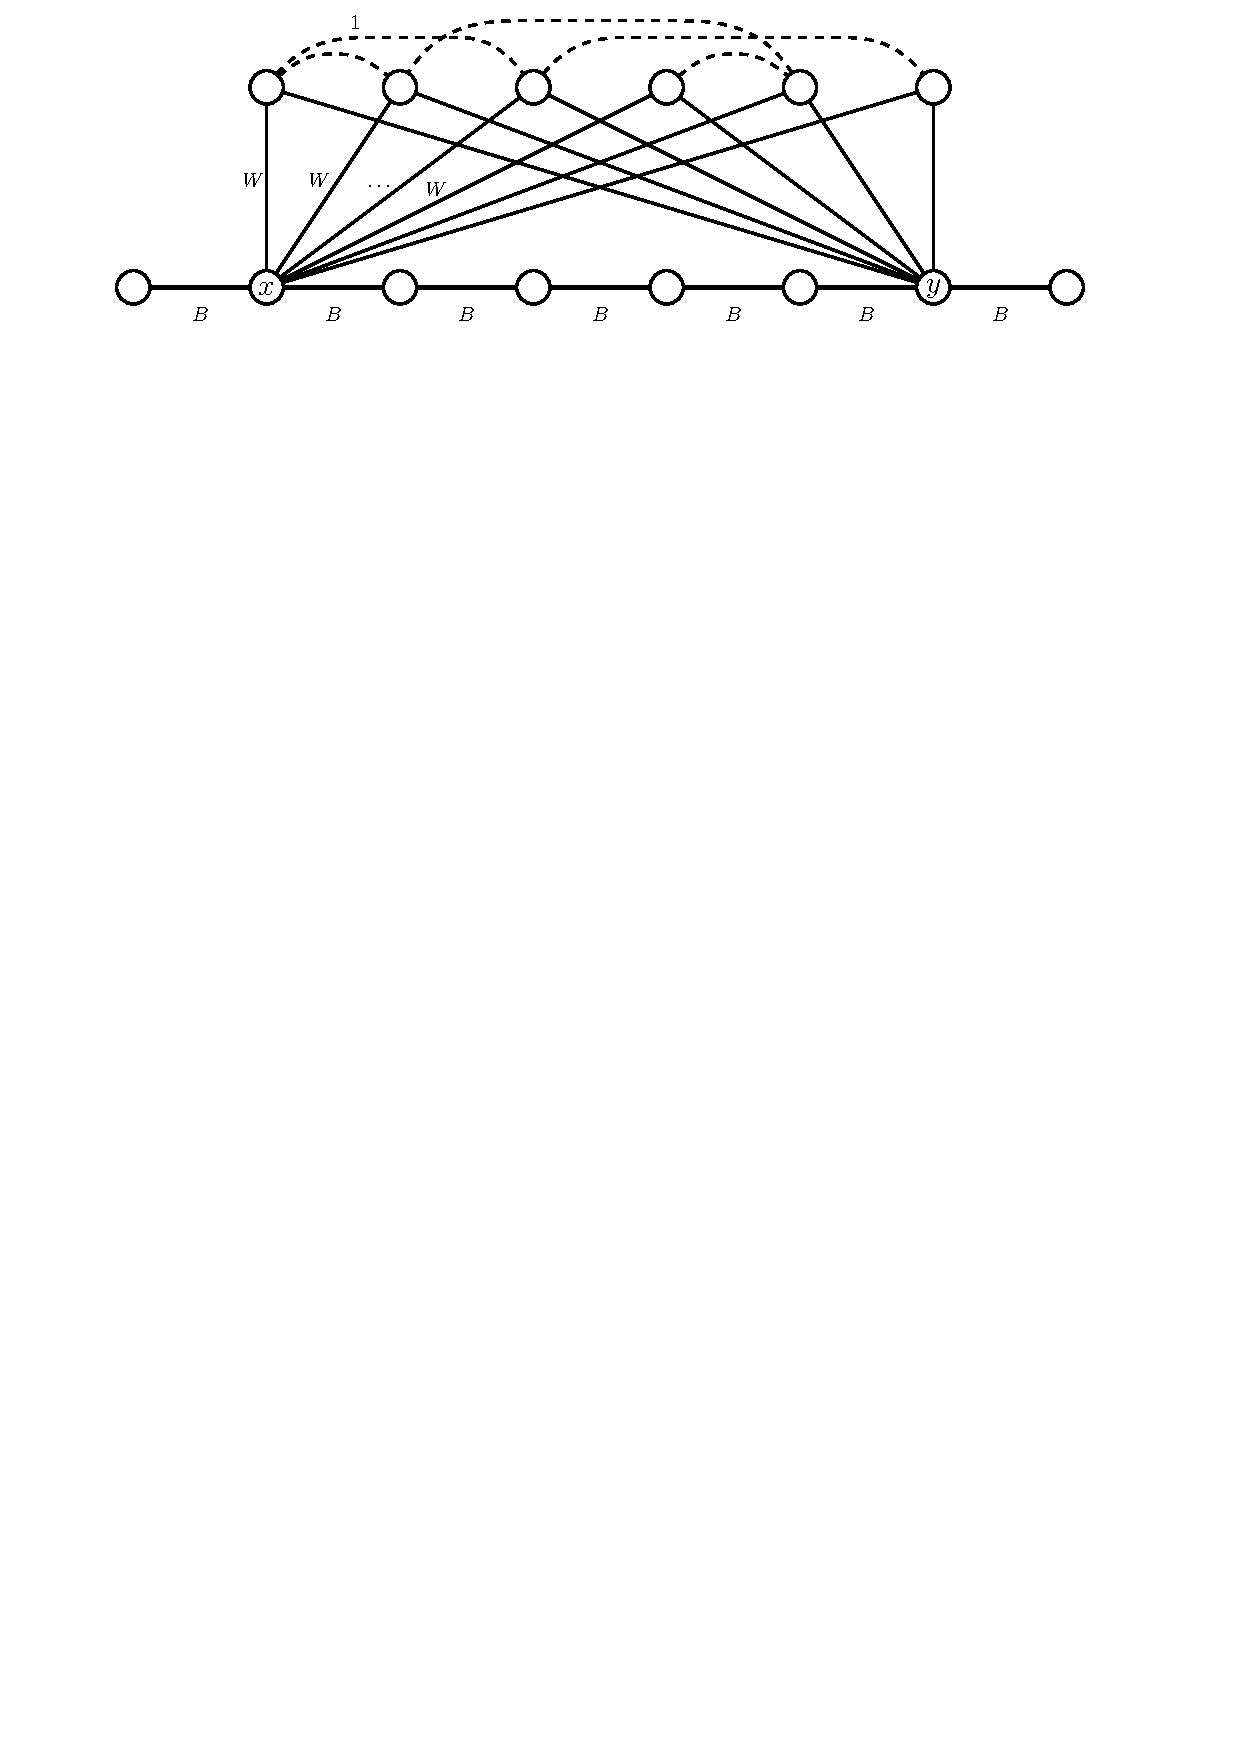
\includegraphics[width=0.3\textwidth]{figs/substitute}
	\caption{Example figure of the construction of the LB and growing components.}
	\label{fig:nptree-construction}
\end{figure}


The adversary constructs ground sets (a set of nodes that may communicate, see Section~\ref{sec:prelim}) depending on choices of a deterministic online algorithm.
We emphasize that the algorithm does not know ground sets before they are revealed.
Once we construct a ground set, it lasts until the end of the input sequence.

The constructed ground sets can be perfectly partitioned into the clusters (i.e., with nodes of each ground set collocated).
This way, the optimal algorithm moves to a perfect partition at the beginning (where requests incur the cost~$0$), thus its cost is bounded.
If the algorithm splits any pair of nodes of a ground set, the adversary issues requests to any pair of split nodes.
These two observations imply that the algorithm must eventually collocate all nodes of a~ground set to be competitive.

First, we construct a ground set of size $k-1$ on an arbitrary cluster $S$.
In any configuration, there exists an alone node on $S$.
We issue requests between the current alone node from $S$, and some node that was initially collocated with it.
Repeating such requests, almost all the nodes must visit the cluster $S$.
In comparison, \OPT performs only two migrations.

\begin{theorem}
	\label{th:lowerbound}
	The competitive ratio of any deterministic online algorithm for \OBRP is at least $(k\cdot \ell - k - \ell)/2$ for any $k\geq 3$ and $\ell \geq 2$.
\end{theorem}

\begin{proof}
	Fix any online algorithm \ALG{}.
	Let $I(C)$ denote the cluster where nodes of the ground set $C$ are located initially.
	If $C$ contains nodes that originate from different clusters, $I(C)$ is undefined.
	\mahmoud{i.e., $I(C):=...$formalized with notations}.
	Throughout the construction, we maintain ground sets for each node.
	Initially all nodes are \emph{alone} (they belong to their own trivial ground sets).
\mahmoud{isolated would be a better word for "alone"}
	First, we create a ground set of size $k-1$ on an arbitrarily chosen cluster $S$.
	\mahmoud{$\mathcal{S}$ is better for a set of sets.}
	%We never dismiss any constructed ground set.
	Each cluster hosts exactly $k$ nodes, and in any configuration a single alone node resides in $S$. \mahmoud{an isolated node is collocated with  this GS in $\mathcal{S}$. We denote the first such node by $x_0$.}

	Then, we add the alone node from $S$ to a larger ground set to force its eviction.
	Precisely,
	we create a ground set $\{x_0, y_0\}$, 
	where $x_0$ is the alone node from $S$ and $y_0$ is an arbitrary node that does not reside in $S$.
	\ALG has them split, and the adversary issues external requests until \ALG collocates them.
	The cluster $S$ already contains a ground set of size $k-1$, hence \ALG must collocate $\{x_0, y_0\}$ in another cluster.
	To preserve a feasible partition of nodes into clusters after collocating $\{x_0, y_0\}$,
	\ALG must replace $x_0$ with another single node.
	\mahmoud{In any new partition, \ALG must replace $x_0$..., otherwise it is not a feasible partition.}
	

	We continue adding the node that is currently alone in $S$ to a larger ground set.
	Precisely, for an alone node $x$ from~$S$, we merge the ground sets of $x$ and the largest ground set $C$ s.t. $C \neq \{x_0,y_0\}$ and $I(C) = I(x)$.
	\mahmoud{$x_i$?}
	This way, $x$ is evicted similarly to $x_0$, and we continue creating such ground sets.
	We describe the termination condition shortly.
	(Note that these ground sets contain nodes that originate from the same cluster, whereas the nodes $x_0$ and $y_0$ originate from distinct clusters.)

	We claim that expanding ground sets in this way can continue as long as at least $\ell$ alone node exists.
	Fix the moment just before the creation of a ground set with the alone node \mahmoud{$x_{t^*}$?} that currently resides in $S$.
	\mahmoud{ALG might change $S$. We can say, "currently collocated with the...".}
	We show that if at least $\ell$ alone nodes exists (including $z$), then there exists a perfect partition of ground sets after expanding a ground set with $z$.
	\mahmoud{the termination condition is needed before the claim statement.}
	To show this claim, we consider a configuration, where the largest ground set of each cluster originates from it (excluding the ground set $\{x_0, y_0\}$).
	In this configuration, each cluster contains:  at most one ground set larger than $1$, possibly some alone nodes, and possibly the ground set $\{x_0, y_0\}$.
	If $I(z)$ contains an alone node, then we simply obtain a~perfect partition by swapping it with $z$.
	In the following we assume that no alone nodes exist on $I(z)$.
	The largest ground set of $I(z)$ is at most $k-1$, because $z$ is on $S$.
	Therefore $\{x_0, y_0\}$ is present on $I(z)$, and we must evict it to make space for $z$.
	To find the cluster for $\{x_0, y_0\}$, observe that we have at most $\ell-1$ clusters with alone nodes, and we have at least $\ell$ alone nodes --- hence a cluster with two alone nodes exists.
	To find a feasible partition, we swap $\{x_0, y_0\}$ with these two collocated alone nodes, and then we swap an alone node from $I(z)$ with $z$.
	

	To keep \OPT's cost low, we end extending ground sets prematurely --- while there are still $\ell+1$ alone nodes (i.e., neglecting two last ground set expansions).
	Consider \ALG's configuration after the last expansion.
	Among $\ell+1$ alone nodes there must exist a pair that originates from the same cluster (we have $\ell$ clusters). 
	We denote these two nodes by $x^*$ and $y^*$.

	The optimal strategy is to perform two node swaps.
	Precisely, \OPT collocates $\set{x_0,y_0}$ by swapping them with $x^*$ and $y^*$.
	In this configuration, no ground set is split.
	We never issue requests between nodes $x^*, y^*$ that are split in this configuration.


	\ALG performs at least one swap for every expansion of a ground set.
	Each expansion reduces the number of alone nodes by $1$.
	We start with $k \cdot \ell - (k-1)$ alone nodes (a single $k-1$ ground set is revealed prior to $\{x_0, y_0\}$), and we end with alone $\ell+1$ nodes.
	The competitive ratio is then $\ALG / \OPT \geq (k\cdot \ell - k - l) / 2$.
\end{proof}


\noindent
\textbf{General partitioning problem.}
Every lower bound for the learning problem constitutes a converging lower bound for the partitioning problem as the input sequence grows to infinity.
However, our construction allows for an exact lower bound for partitioning with finite input sequence.
To this end, we issue only enough requests until the algorithm collocates the nodes of each ground set (if it never does, we terminate after it pays $k\cdot \ell$).
The construction is oblivious to the choice of the reconfiguration cost $\alpha$: we compare the 	number of node exchanges of \ALG and \OPT.



\noindent
\textbf{Resource augmentation.}
The majority of work on Online Balanced Partitioning so far \cite{repartition-disc,sigmetrics19_partitioning} focuses on the scenario with resource augmentation, where the clusters of \ALG are larger than the clusters of \OPT.
We can adjust our construction to show a lower bound of $\Omega(\ell)$ for resource augmentation.

Consider a partitioning problem with resource augmentation $1+1/3-\epsilon$.
Fix $k$ divisible by $3$, and construct $3$ ground sets of size $k/3$ in each cluster.
Note that no more than $3$ such ground sets fit in one cluster.
Then, apply the construction from the lower bound for $k=3$, using these ground sets in the way we used individual nodes.
The cost of any algorithm (including \OPT) scales up by $k/3$, and the lower bound $\Omega(\ell)$ holds.

Finally, we note the possibility for improvement. The algorithm CREP~\cite{repartition-disc} requires $(2+\epsilon)$-augmentation to guarantee the competitive ratio independent of $\ell$.

\subsection{Upper bound.}
\label{sec:ppl}

We present an asymptotically optimal algorithm for the learning problem.
The algorithm immediately collocates every communicating pair and never separates them.
In other words, it maintains components, introduced in the preliminaries (Section~\ref{sec:prelim}).

Upon receiving any external request, two components merge --- and this requires a reconfiguration.
Many configurations may be feasible, and we choose the one that is \emph{closest to the initial configuration}.

\maciek{The remainder of the paper used "configuration C" to denote the partition P. Easiest to adjust here.}

\noindent
\textbf{Perfect Partition Learner algorithm.}
Fix the initial configuration
$P_I = I_1, \dots, I_{\ell}$ and \OPT's final configuration
$P_F = F_1, \dots, F_{\ell}$\maciek{How do we define a configuration?}.
The \emph{distance} of a configuration $P = C_1, \dots, C_{\ell}$ from the initial configuration \maciek{, denoted $\dist(P)$} is the number of nodes in $P$ that do not reside in their initial cluster.
\maciek{We might denote distance $\Delta(P)$, and the current $\Delta$ might be R (like radius).}
That is,
$\dist(P, P_I) := \sum_{j=1}^{\ell} | C_j \setminus I_j |$
\maciek{Major: what does this definition mean? This is highly unclear, most likely because a configuration was not defined.}. 
In other words,
at least $\dist(P, P_I)/2$ node swaps are required in order to reach the configuration $P$ from $P_I$, and thus
$\OPT \geq \Delta:= \dist(P_F, P_I) $.
With each repartitioning,
\PPL moves to a configuration that minimizes the distance to the initial configuration $P_I$.
As a result,
\PPL never ends up \maciek{ends up is informal} in a configuration that is more than $\Delta$ (single-node) migrations away from $P_I$ \maciek{This is not an algorithm definition, that's its property. Should not be in this paragraph}.
This invariant ensures that \PPL does not pay too much while recovering $P_F$ \maciek{Recovering $P_F$? It's not the goal. At least at this point the reader is confused: it does not know yet that PPL is proven to end up in $P_F$}.
%      \maciek{``re-partition'' procedure name should indicate the fact that this is a specific repartition that is close to initial partition}
We note \maciek{Define?} that the $\mathit{repartition}$ at Line \ref{line:rebalance} replaces the current configuration $P$ with a~perfect partition closest to $P_I$.
Hence it never moves to a configuration beyond distance $\Delta$ \maciek{This is again mixing the properties of ppl and its definition. Restructure}.
The scheme of the algorithm can be found in the Algorithm \ref{alg:PPL}.

\section{PPL Algorithm} \label{alg:PPL}
\begin{algorithm}
	\renewcommand{\algorithmicrequire}{\textbf{Input:}}
	\renewcommand{\algorithmicensure}{\textbf{Output:}}
	\begin{algorithmic}
		%        \Require 
		%        $k, \ell$,
		%        initial configuration $P_I$,
		%        sequence of  requests $\sigma_1, \dots, \sigma_N$ 
		%        \Ensure A final configuration $P_F$ 
		\STATE {For each node $v$ create a singleton component $C_v$ and add it to $\mathcal{C}$}
		\STATE{$P_0 := P_I$}
		\label{line:initcomponents}
		\FOR {each  request $\sigma_t=\{u,v\}, 1 \leq t \leq N$}
		\STATE Let $C_1 \ni u$ and $C_2 \ni v$ be the container components
		\IF{$C_1 \neq C_2$}
		\STATE {Unite the two components into a single component $C'$ and
		$\mathcal{C} = (\mathcal{C}\setminus\set{C_1, C_2}) \cup ~\set{C'}$} \label{line:mergecomponents}
		\IF{$\mathit{cluster}(C_1, P_{t-1}) \neq \mathit{cluster}(C_2, P_{t-1})$
		\COMMENT{i.e.~if not in the same cluster}    
		}       
		\STATE {$P_{t} = \mathit{repartition}(P_{t-1}, P_I, \mathcal{C})$} 
		\COMMENT{move to $P$ closest to $P_I$}
		\label{line:rebalance} 
		\ENDIF
		\ENDIF
		\ENDFOR
	\end{algorithmic}
	\caption{Perfect Partition Learner (\PPL)}
	\label{alg:ppl}
\end{algorithm}


\maciek{Algorithm pseudocode comments}
\maciek{Major thing to discuss: do we even need this? The algorithm is very simple, and the description in the paragraph would be much better. The only way to save it would be to have a general algorithm pseudocode (equivalent to DET), and parametrize it with the repartition procedure. Here, we would say that we choose the closest to initial, and it ALG3 we say that we choose the closest to current.}
\maciek{This is not good that we need a comment about what $cluster \neq cluster$ means}
\maciek{In pseudocode we need extremely short sentences. $C := singleton components ... $?; $Merge C, C'$ etc}
\maciek{No need to maintain $P_i$'s. Just use one $P$? Or without naming: "move to partition (closeToInit(...))", and remove the partition args from cluster().}
\maciek{Online algorithms should have different pseudocode. Instead of for loop, start with "When a request u,v arrives" (before that it is ok to have init phase just like it is now)}

\begin{property} \label{prop:dist<OPT}
	Let $P$ be any configuration chosen by \PPL at Line $\ref{line:rebalance}$.
	Then, $\dist(P,P_I) \leq \Delta$.
	\maciek{Express the configuration without refering to pseudocode?}
\end{property}
\maciek{The property is explained in the previous paragraph. Here, reader thinks that this is obvious and wonders why. Restructure: Move closer to the exlaination text. Or even make this property a lemma (most likely better).}

\begin{lemma}	\label{lemma:rebalancecost}
	The cost of repartitioning at Line \ref{line:rebalance} is at most $2\cdot\OPT$.
	\maciek{Express the reconfiguration without pseudocode?}
\end{lemma}
\begin{proof}
	Consider the repartitioning that transforms $P_{t-1}$ to $P_t$ upon the request $\sigma_t$.
	Let $M \subset V$ denote the set of nodes that migrate during this process.
	Let $M^-$ and $M^+$ denote the subset of nodes that (respectively)
	enter or leave their original cluster during the repartitioning.    
	Then,
	$M = M^+ \cup M^-$.
	Since \maciek{at least?} $|M^-|$ nodes are not in their original cluster before the repartitioning (i.e., in $P_{t-1}$),
	the distance before the repartitioning is $\dist(P_{t-1},P_I) \geq | M^-|$.
	Analogously,
	the distance afterwards is $\dist(P_{t},P_I) \geq | M^+|$.
	Thus,
	$|M| \leq \dist(P_{t-1},P_I) + \dist(P_{t},P_I)$.
	By Property \ref{prop:dist<OPT},
	$\dist(P_{t-1},P_I) , \dist(P_{t},P_I) \leq \Delta \leq \OPT$
	and thereby we have	
	$|M| \leq 2\cdot\OPT$.
	\maciek{the comma between $\dist$ is confusing. BOTH are bounded? If so, expand the sentence and write both individual bounds.}
\end{proof}

\begin{theorem}	\label{thm:upperbound}
	\PPL reaches the final configuration $P_F$ and it is $(2\cdot k\cdot\ell)$-competitive.
	\maciek{Do not hide that we have $2(k-1)\ell$ in the theorem. This is a better bound.}
\end{theorem}
\begin{proof}
	On each inter-cluster request,
	the algorithm enumerates all $\ell$-way partitions of components
	that are in the same (closest) distance of $P_I$.
	That is, 
	once it reaches a configuration $P$ at distance $\Delta = \dist(P, P_I)$,
	it does not move to a configuration
	$P', \dist(P', P_I) > \Delta$,
	before it enumerates all configurations at distance $\Delta$.
	Therefore,
	\PPL eventually reaches $\Delta=\OPT$ and the configuration $P_F$.
	%    including the request that completes revealing of all components that are collocated in $P_F$.
	There are at most $(k-1)\cdot\ell < k\cdot\ell $ calls   to $\mathit{repartition}$
	(i.e., the number of internal edges in $P_F$).
	\maciek{Clarify why the number of internal edges bound the number of repartitions.}
	By Lemma \ref{lemma:rebalancecost},
	each repartition costs at most $2\cdot\OPT$.
	The total cost is therefore at most $2\cdot\OPT\cdot k\cdot\ell$, which implies the competitive ratio.
	%    \mahmoud{This is the cost of moving and the cost of remote comm. is not counted.
	%    	So it is 4-competitive (?)}
\end{proof}

% In Section~\ref{sec:lowerbound} we constructed a $\Omega(k \cdot \ell)$ for \OBRP{}.
% Note that the lower bound holds also in the perfect partition model, as the constructed input sequence allows \OPT to move to a perfect partition.
% The corollary is that PPL is optimal.

\section{The Partitioning Problem}
\label{sec:part}



\maciek{Start with referencing the table of results, saying that some results are known already in the literature. And emphasize here that we now have an improved lower bound from the previous section, as that model was a subproblem.}

Let us now discuss the general online
model where the request sequence
can be arbitrary.
We show that the classic \emph{rent-or-buy} approach~\cite{karlin-ski-rental} allows obtaining an optimal algorithm for $k=3$.
Upon receiving $\alpha$ requests between a pair of nodes, we collocate them in one cluster until the end of a phase (that we define precisely later).

\maciek{Rewrite above paragraph to say that our algorithm is essentially DET from DISC16, with concretised reconfiguration strategy (i.e., an arbitrary one among the minimum cost reconfigurations)}

\maciek{Better name than DET? Currently it is \TAlg, hence it is wrong}

\subsection{Improved analysis of the component-based algorithm}
\label{sec:k3}


%We define the algorithm \TAlg in the following way.
Now we describe the algorithm \TAlg.
It partitions nodes into components, and
initially, each node belongs to its own singleton component.
For each pair of nodes, \TAlg maintains a counter, initiated to $0$. 
Upon receiving a request to a pair that is not collocated in one cluster, it increases their counter by $1$.
If the counter for a pair $(u,v)$ reaches $\alpha$, \TAlg merges the components of $u$ and $v$, and moves to the closest component respecting partitioning.
If no such partitioning exists, \TAlg resets all components to singletons, resets all counters to $0$, and ends the phase.

\maciek{Emphasize the difference to DET: "Modification is the following: when repartition is necessary, move to \emph{the closest} perfect partition of components."}




\begin{figure}[H]
	\centering
	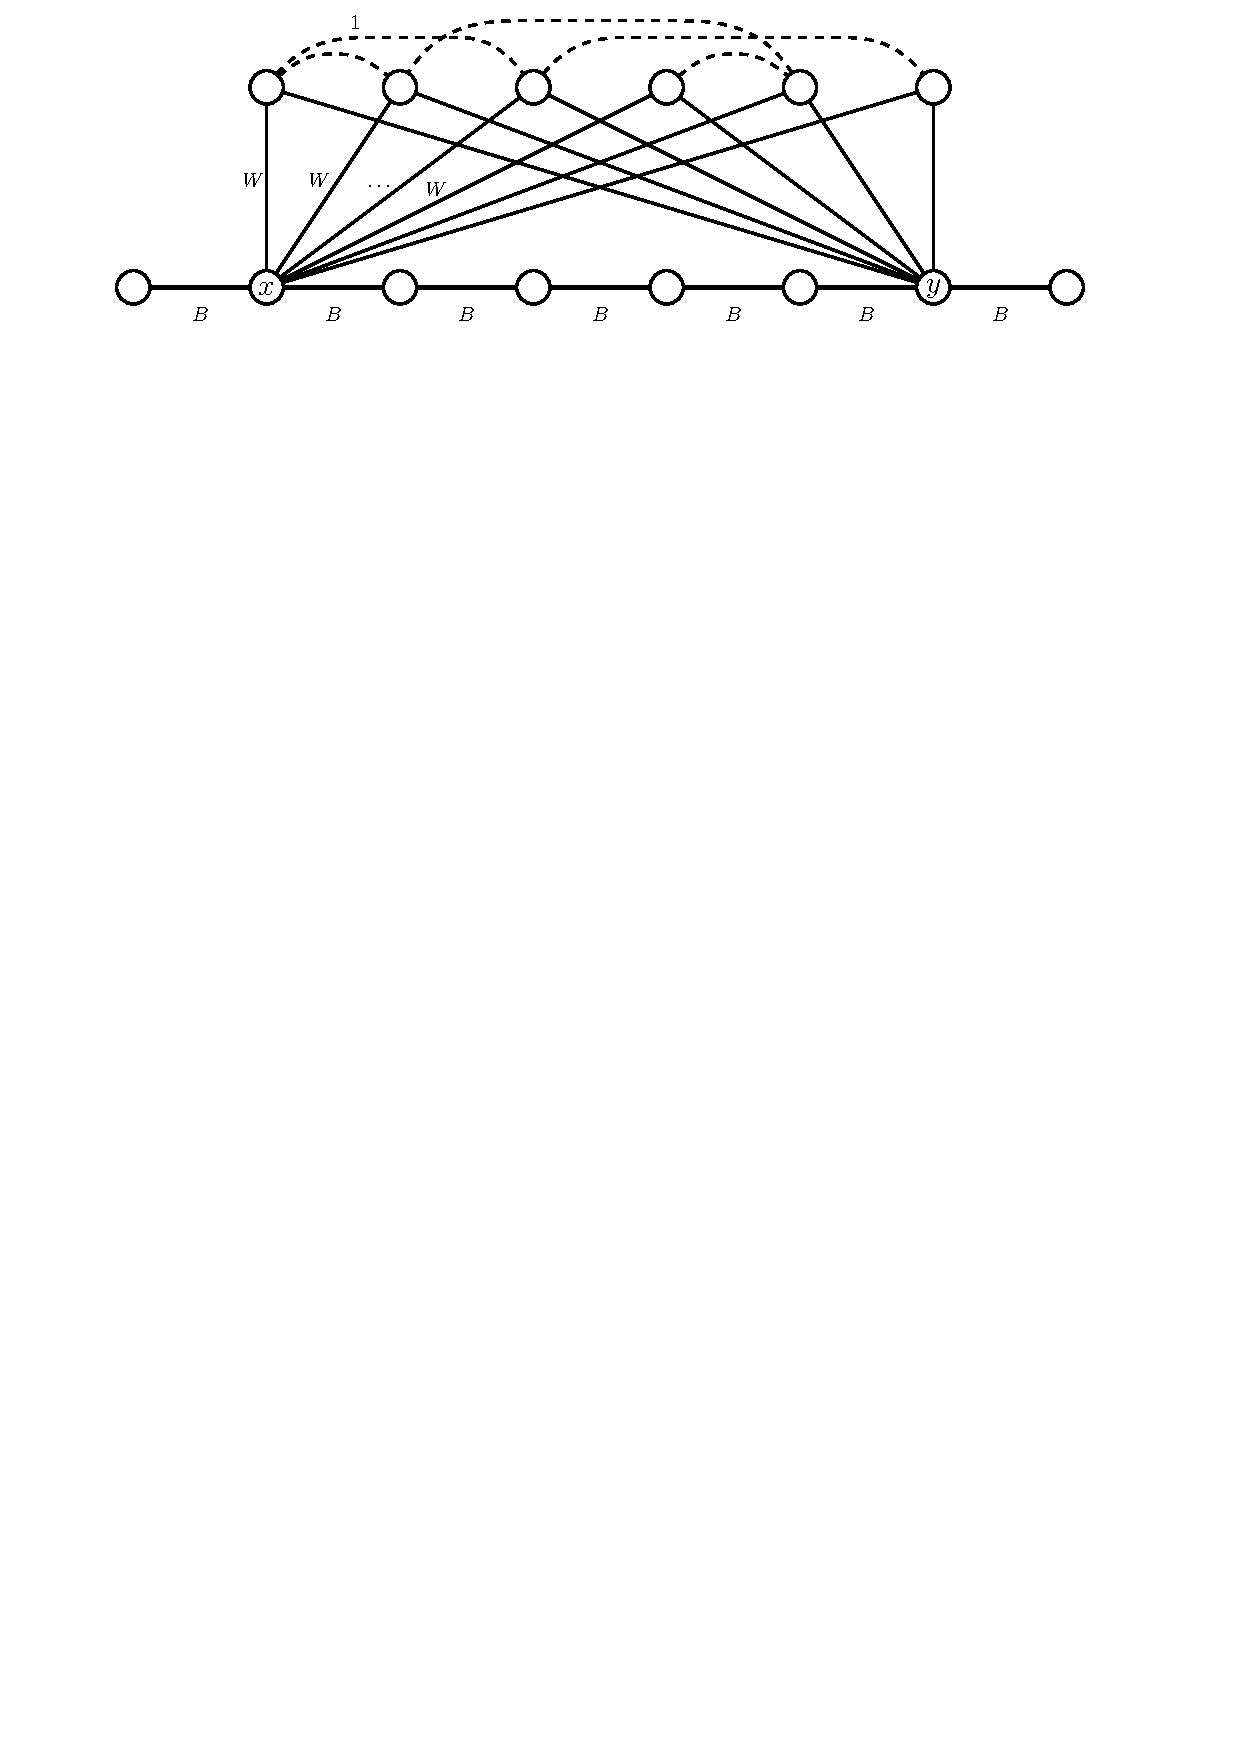
\includegraphics[width=0.3\textwidth]{figs/substitute}
	\caption{an unsaturated edge that is inside a component}
\end{figure}



\begin{theorem}
	\TAlg is $O(\ell)$-competitive.
	\maciek{Proposed new formulation (current version is all about k=3 still): Let Reconf(k,l) be a bound on the cost of a single reconfiguration. Then \TAlg is $O(Reconf(k,l)\cdot k \cdot \ell)$-competitive.}
\end{theorem}
\begin{proof}
	Fix a completed phase, and consider the state of \TAlg's counters at the end of it.
	We consider the incomplete phase later in this proof.
	
	As \TAlg is component respecting, it never increases any counter above $\alpha$.
	We say that the pair $(u, v)$ is \emph{saturated} if the counter has value $\alpha$, and \emph{unsaturated} otherwise \maciek{Rename: saturated/unsaturated edge instead of a pair}.
	Let $\sigma$ be the input sequence that arrived during the phase.
	Let $\sigma_{cost}$ be the requests that at the moment of arrival were external requests for \TAlg (these are the only requests that incurred a cost for \TAlg).
	In our analysis, we partition $\sigma_{cost}$ into subsequences $\sigma_I$ and $\sigma_E$.
	The sequence $\sigma_I$ (inter-component requests) are the requests from $\sigma_{cost}$ issued to pairs that belong to the same component of \TAlg at the end of the phase.
	The sequence $\sigma_E$ (extra-component requests) denotes the requests from $\sigma_{cost}$ that do not appear in $\sigma_I$.
	
	
	%Let $A^I$ be the cost of (extra-cluster) communication incurred in this phase by \TAlg between pairs that belonged to the single component at the end of the phase.
	%Let $A^E$ be the cost of (extra-cluster) communication incurred in this phase between the nodes that belong to different components at the end of this phase.
	Let $\TAlg(M)$ be the cost of migrations performed by \TAlg in this phase.
	\TAlg performs at most $2 \ell$ component merge operations, as
	exceeding this number means that a component of size $4$ exists, and the phase should have ended already.
	Combining this with Lemma~\ref{lem:1req} gives us $\TAlg(M) \leq 8\alpha\cdot\ell$ (recall that an exchange costs $2\alpha$).
	%Together with Lemma~\ref{lem:1req}, this allows us to bound the cost of migrations, $\TAlg(M) \leq 6\cdot\alpha\cdot\ell$.
	
	Now we bound $\TAlg(\sigma_I)$.
	A~cluster of type $C_3$ contributes at most $3 \alpha - 1$ to $\TAlg(\sigma_I)$, as $2$ of pairs of nodes from the component are saturated and contribute $\alpha$ each, and the third, unsaturated pair contributes at most $\alpha-1$.
	Other cluster types contribute less: $C_1$ contributes $0$ and $C_2$ contributes $\alpha$.
	Summing this over all $\ell$ clusters gives us $\TAlg(\sigma_I) \leq (3 \alpha-1)\cdot \ell \leq 3\alpha\cdot\ell$.
	
	%We bound $A^E$ by $k^2 \cdot (\alpha - 1)$, as no more than $k^2$ pairs are unsaturated, and each of them contributes at most $\alpha -1$.
	%\maciek{not needed most likely}
	
	Moreover, \TAlg paid for all requests from $\sigma_E$, and thus $\TAlg(\sigma_E) = |\sigma_E|$.
	In total, the cost of \TAlg is at most $\TAlg(\sigma_I) + \TAlg(\sigma_E) + \TAlg(M) \leq 11\alpha\cdot \ell + |\sigma_E|$ during this phase.
	
	\medskip
	
	Now we lower-bound the cost of $\OPT$.
	By $\OPT(\sigma_I)$ and $\OPT(\sigma_E)$ we denote the cost of $\OPT$ on these input sequences (defined with respect to components of \TAlg in this phase).
	By $\OPT(M)$ we denote the cost of migrations performed by $\OPT$ in this phase.
	
	We split the cost of $\OPT$ into parts coming from serving $\sigma_I$ and $\sigma_E$.
	While serving these requests, $\OPT$ may perform migrations, and we account for them in both parts: we separately bound $\OPT$ by $\OPT(\sigma_I) + \OPT(M)$ and $\OPT(\sigma_E) + \OPT(M)$.
	Combining those bounds gives us $\OPT \geq \max\{\OPT(\sigma_I) + \OPT(M), \OPT(\sigma_E) + \OPT(M)\} \geq (\OPT(\sigma_I) + \OPT(M)) / 2 + (\OPT(\sigma_E) + \OPT(M)) / 2$.
	
	%Let $O^M$ be the cost of migrations performed by $\OPT$ during the phase.
	%Let $O^I$ be the cost of serving requests between nodes that were put in one component by \TAlg during this phase.
	%Let $O^E$ be the cost serving requests between nodes that \TAlg did not put in the same component during that phase.
	
	%First, we estimate the cost related to $\sigma_I$.
	We have $\OPT(M) + \OPT(\sigma_I) \geq \alpha$, as the phase ended when the components of \TAlg{} could not be partitioned without splitting them.
	Hence, for every possible configuration of $\OPT$, there exists a non-collocated pair of nodes with at least $\alpha$ requests between them, and
	$\OPT$ either served them remotely or performed a~migration.
	
	\medskip
	Before we bound the competitive ratio, we relate the costs of $\TAlg$ and $\OPT$ with respect to requests $\sigma_E$.
	In a~fixed configuration of $\OPT$, it may mitigate paying for requests between at most $3\ell$ pairs of nodes by collocating them in its clusters.
	Recall that $\sigma_E$ consists of requests to unsaturated pairs, and it accounts only for requests that increased the counter (i.e., external requests), thus $\OPT$ may mitigate at most $3\ell\cdot(\alpha - 1)$ requests from $\sigma_E$.
	Faced with $W := |\sigma_E| - 3\ell\cdot(\alpha-1)$ requests $\sigma_E$ that it could not mitigate, $\OPT$ served some of them remotely and possibly performed some migrations to decrease its cost.
	
	
	Now we estimate the cost of $\OPT(\sigma_E)$ while accounting savings from migrations.
	By performing a swap of nodes $(u,v)$, $\OPT$ collocates $u$ with two nodes $u', u''$, and $v$ with two nodes $v'$, $v''$.
	This may allow serving requests between $(u,u')$, $(u,u'')$, $(v,v')$ and $(v,v'')$ for free afterwards.
	As $\sigma_E$ consists of requests to unsaturated pairs, and it accounts only for external requests, there are at most $\alpha-1$ requests between each of these pairs.
	By performing a single swap that costs $2\alpha$, $\OPT$ may avoid paying the remote serving costs for at most $4 (\alpha - 1)$ requests from $\sigma_E$
	\maciek{This changes in the general case, and introduces the factor $~1/k$ in opt's cost, increasing the competitive ratio by $O(k)$}.
	Thus, for serving $\sigma_E$, $\OPT$ pays at least $\OPT(\sigma_E) + \OPT(M) \geq W \cdot \frac{2\alpha}{4 (\alpha-1)}\geq |\sigma_E| / 2 - 2 \alpha \cdot \ell$.
	From that, we obtain $|\sigma_E| \geq 2(\OPT(\sigma_E)+\OPT(M)) + 4\alpha \cdot \ell$.
	Let $E := \OPT(\sigma_E) + \OPT(M)$. Finally, we are ready to bound the competitive ratio
	\begin{equation*}
		\frac{\TAlg(\sigma)}{\OPT(\sigma)} \leq \frac{11\alpha \cdot \ell + |\sigma_E|}{\alpha/2 + E/2} \leq \frac{27\alpha\cdot\ell + 2\cdot E}{\alpha + E} \leq 27 \ell = O(\ell).
	\end{equation*}
	
	\medskip
	
	It remains to consider the last, unfinished phase.
	Consider the case, where the unfinished phase is also the first one.
	Then, we cannot charge $\OPT$ due to the inability to partition the components.
	Instead, we use the fact that \TAlg and $\OPT$ started with the same initial configuration.
	We charge $\OPT$ $\alpha$ for the first external $\alpha$ requests or a migration,
	and we follow the analysis regarding the unsaturated requests.
	If the input finished before the first $\alpha$ external requests, then \TAlg is optimal.
	\maciek{Missing second case: then we just charge opt alpha for this one edge and this is sufficient, as the cost of alg only decreases from the full phase}
	Now, consider the case, where there are at least two phases, then we split the cost $\alpha$ charged in the penultimate phase into last two phases, and follow the analysis regarding the unsaturated requests.
	This way, the competitive ratio increases at most twofold.
\end{proof}


\subsection{Warm-up: bounding the reconfiguration for $k=3$}


\begin{figure}[H]
	\centering
	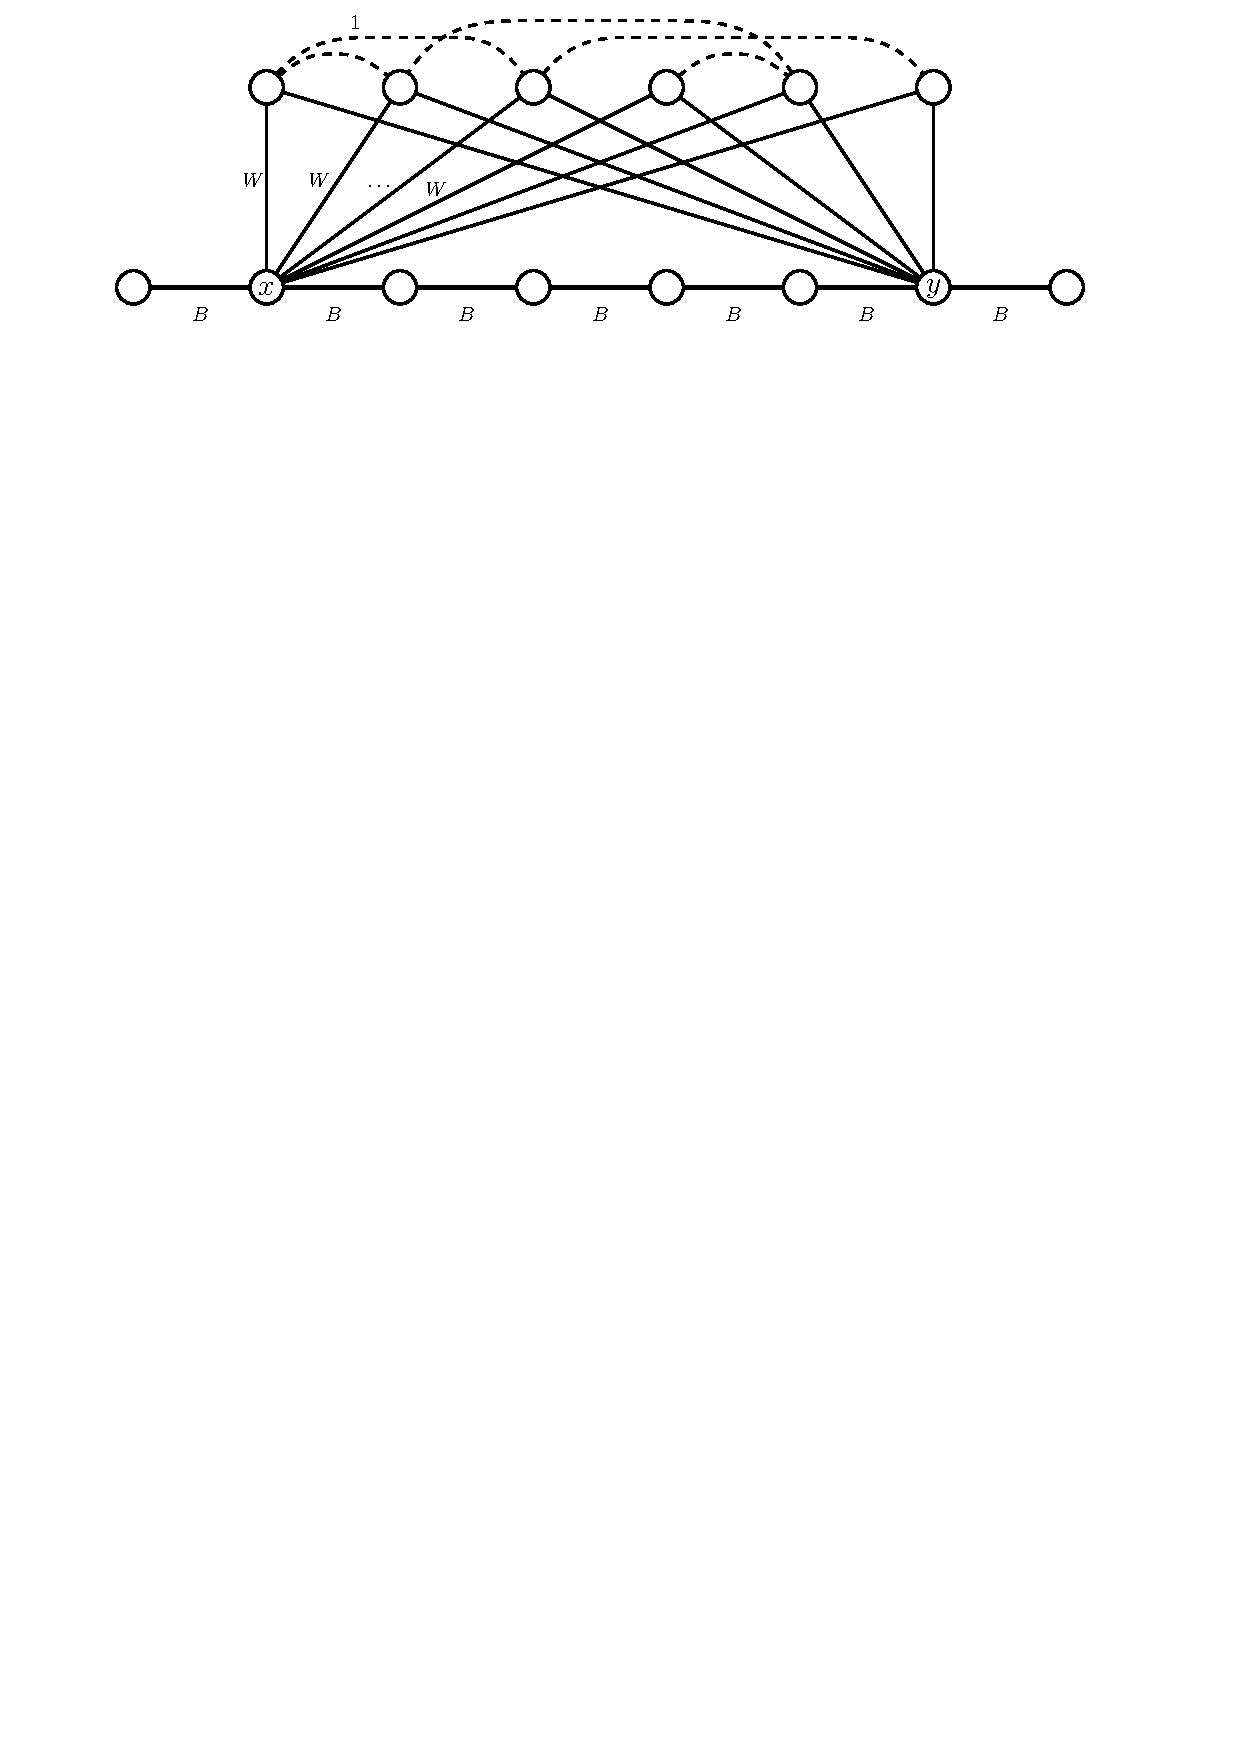
\includegraphics[width=0.3\textwidth]{figs/substitute}
	\caption{Cluster signatures in warm-up k=3 proof}
\end{figure}

\maciek{Rewrite: cluster types should be cluster signatures}
In our analysis, we distinguish among three types of clusters: $C_1, C_2, C_3$. In a cluster of type $C_i$, the size of the largest component contained in this cluster is $i$.
Before bounding the competitive ratio of \TAlg, we introduce the lemma that estimates the cost of a single repartition of \TAlg.

\begin{lemma}
	\label{lem:1req}
	During a single repartition, \TAlg exchanges at most $2$ pairs of nodes.
\end{lemma}

\begin{proof}
	Observe that when the repartition is triggered by \TAlg, the resulting partitioning is component respecting.
	Otherwise, if it does not exist, \TAlg simply ends the phase and performs no repartition.
	
	%We distinguish between three types of clusters: $C_1, C_2, C_3$,
	%which we define as follows.
	%A cluster of type $C_1$ the cluster contains $3$ singleton components (this is also the initial configuration of any cluster).
	%A cluster of type $C_2$  contains one component of size $2$ and one component of size $1$.
	%Finally, a cluster of type $C_3$  contains one component of size $3$.
	
	Consider a request between $u$ and $v$ that triggered the repartition and let $U$ and $V$ be their respective clusters.
	Note that $U\neq V$,
	as otherwise, the request would not trigger a~repartitioning.
	We consider cases based on the types of clusters $U$ and $V$.
	Note that this is impossible that either $U$ or $V$ is of type $C_3$, as otherwise, we merge components of size $3$, and no component respecting partitioning exists, a contradiction.
	If either $U$ or $V$ is of type $C_1$, then this cluster can fit the merged component, and the reconfiguration is local within $U$ and $V$.
	For two clusters, any configuration can be reached within two swaps, due to the fact that clusters are indistinguishable.
	
	Finally, we consider the case where both $U$ and $V$ are of type $C_2$. Note that $(u,v)$ cannot both belong to a component of size $2$, as this would mean that \TAlg has the component of size $4$, a contradiction with the case assumption that the component respecting partitioning exists. 
	Otherwise, if either $u$ or $v$ belongs to a component of size $2$, then it suffices to exchange components of size $1$ between $U$ and $V$.
	Finally, if $u$ and $v$ belong to components of size $1$, then we must place them in a cluster different from $U$ and $V$.
	Note that in such case, a $C_1$-type cluster $W$ exists, as otherwise no component respecting partitioning exists. In this case \TAlg performs one swap, i.e., it exchanges the nodes $u$ and $v$ with any two nodes of $W$.
\end{proof}

Corollary: DET2 is $O(\ell)$-competitive for $k=3$.


\begin{comment}
\section{Bounding the cost of a single reconfiguration of components}

\maciek{Overview of the section, intro. Defer introducing the graph notation, the warm-up does not need it}

\subsection{Characterization of the migration graph}

Consider a component merge action performed by \TAlg that triggers a reconfiguration from a configuration $C_I$ to a configuration $C_F$.
To execute the reconfiguration, the nodes of two non-collocated components migrate to a common cluster.
Each cluster contains exactly $k$ nodes, thus other nodes migrate to take the place of nodes of merged components.
Their place must be occupied, too, and this way a single merge action may trigger migrations in clusters not directly involved in a merge action (for an example, see Section~\ref{ssec:example}). 
Recall that both $C_I$ and $C_F$ are component-respecting configurations, hence a migration of a single node entails migrations of all nodes of its cluster.

In Section~\ref{ssec:cascade}, we upper bound the cost incurred by a reconfiguration that follows a single component merge.
To this end, we introduce a \emph{migration graph} that models the reconfiguration.
In the following, we characterize the structure of the migration graph.

\noindent
\textbf{Vertices of the migration graph and the core vertices.}
The vertices of the migration graph are all $\ell$ clusters of the instance.
We distinguish the \emph{core vertices} that correspond to clusters directly involved in the merge operation: the clusters containing the to-be-merged components in $C_I$ and the cluster containing the merged component in $C_F$.
There are at most $3$ core vertices in each migration graph (at most two components participate in the merge, and these may migrate to a third cluster).

\noindent
\textbf{Edges and their labels.}
The edges of the migration graph denote the migration of nodes from $C_I$ to $C_F$.
Each edge is labeled with a number $m$ that denotes the number of migrated nodes between clusters.
Each edge is directed from the cluster that contained the nodes to the cluster they migrated to.
Both edges might exists between a pair of nodes, as whole components of nodes migrate, and the back-and-forth exchange may be needed for the configuration $C_F$ to be component-respecting.

\noindent
\textbf{Vertex degree.}
At most $k$ nodes may migrate from a cluster and at most $k$ nodes may migrate into a cluster.
Thus, the sum of the labels for both ingoing and outgoing edges of each vertex is at most $k$.
This implies that the number of ingoing and outgoing edges is also bounded by $k$.

\noindent
\textbf{Flow preservation.}
In any feasible configuration, each cluster contains exactly $k$ nodes.
Thus, for any vertex, the sum of labels of ingoing edges must equal the sum of labels of outgoing edges.
\maciek{Can we say that this implies that the graph is a circulation?}

\noindent
\textbf{Migration graph and the cost of reconfiguration.}
The cost of cluster reconfiguration equals the number of exchanged nodes multiplied by $\alpha$.
From the standpoint of a migration graph, this corresponds to the sum of labels on edges of the graph.
A trivial upper bound on the cost is the size of the connected component in the migration graph multiplied by $2\alpha k$.

\medskip

Note that for a single component merge, multiple migration graphs may exist, and multiple of them might have the optimal cost.
In Section \ref{ssec:cascade}, we show that among all migration graphs for given component merge, there exists an optimal graph with the bounded cycle length.
Combined with other properties, this allows to bound the size of the migration graph, and consequently bound the cost of each repartition, that results in a bound of the competitive ratio for \TAlg.

\subsection{Costly cluster reconfiguration example}
\label{ssec:example}



\begin{figure}[H]
	\centering
	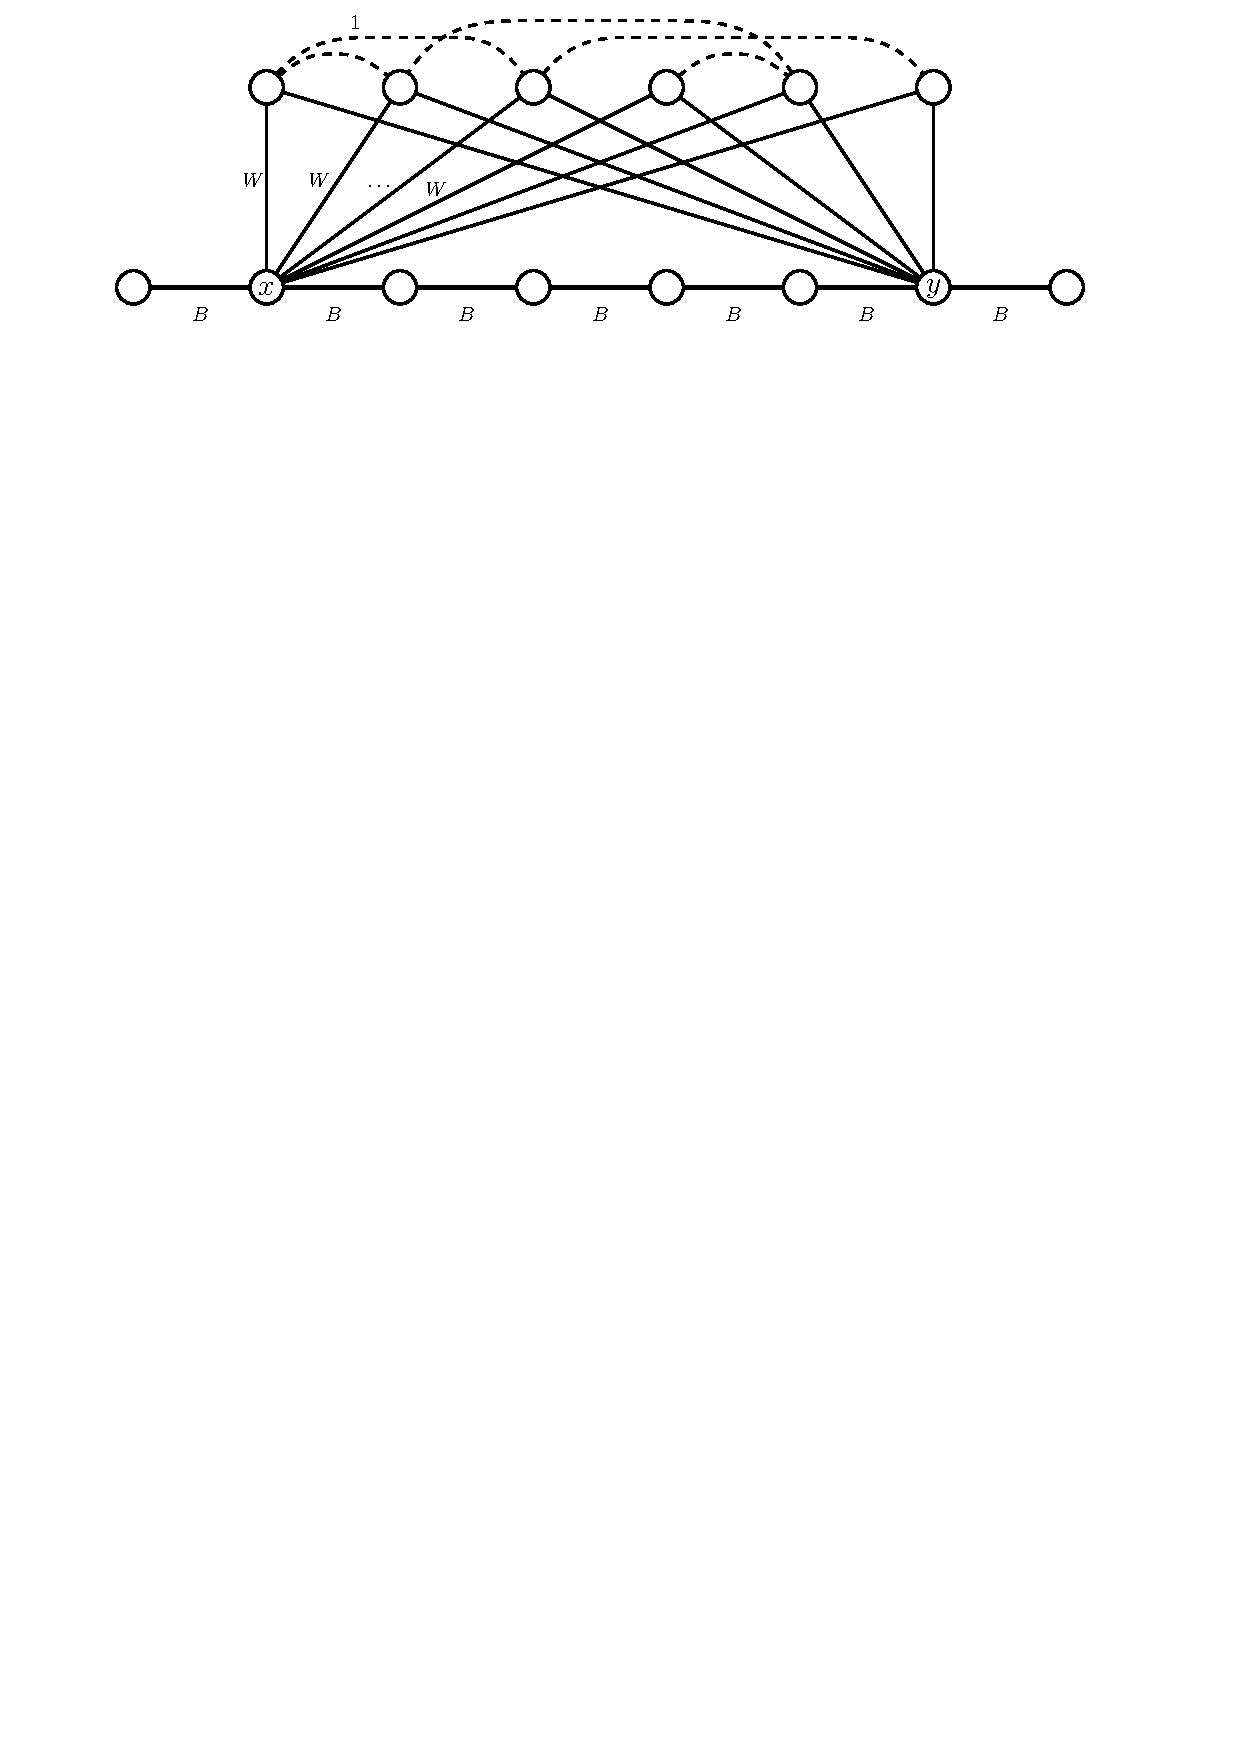
\includegraphics[width=0.3\textwidth]{figs/substitute}
	\caption{A costly cascade example. On the left: the configuration prior to the merge and the merge of two components (denoted solid). On the right: corresponding migration graph for the optimal (unique) reconfiguration.}
\end{figure}


In this section we present an example of a merge action that results in a $k/3$(?) length cycle in an optimal migration graph.

\subsection{Bounds on the size of a migration graph}
\label{ssec:cascade}

In \cite{repartition-disc}, authors trivially bounded the reconfiguration cost for each merge action by $k \cdot \ell$.
This roughly corresponds to migrating every node in every cluster.
Now, we bound the cost of a single repartition of \TAlg as a function of $k$.
Note that the bound of $k \cdot \ell$ is still valid, and the resulting bound is the minimum of these two.

We begin, by bounding the length of each cycle in one of optimal solutions.


\begin{figure}[H]
	\centering
	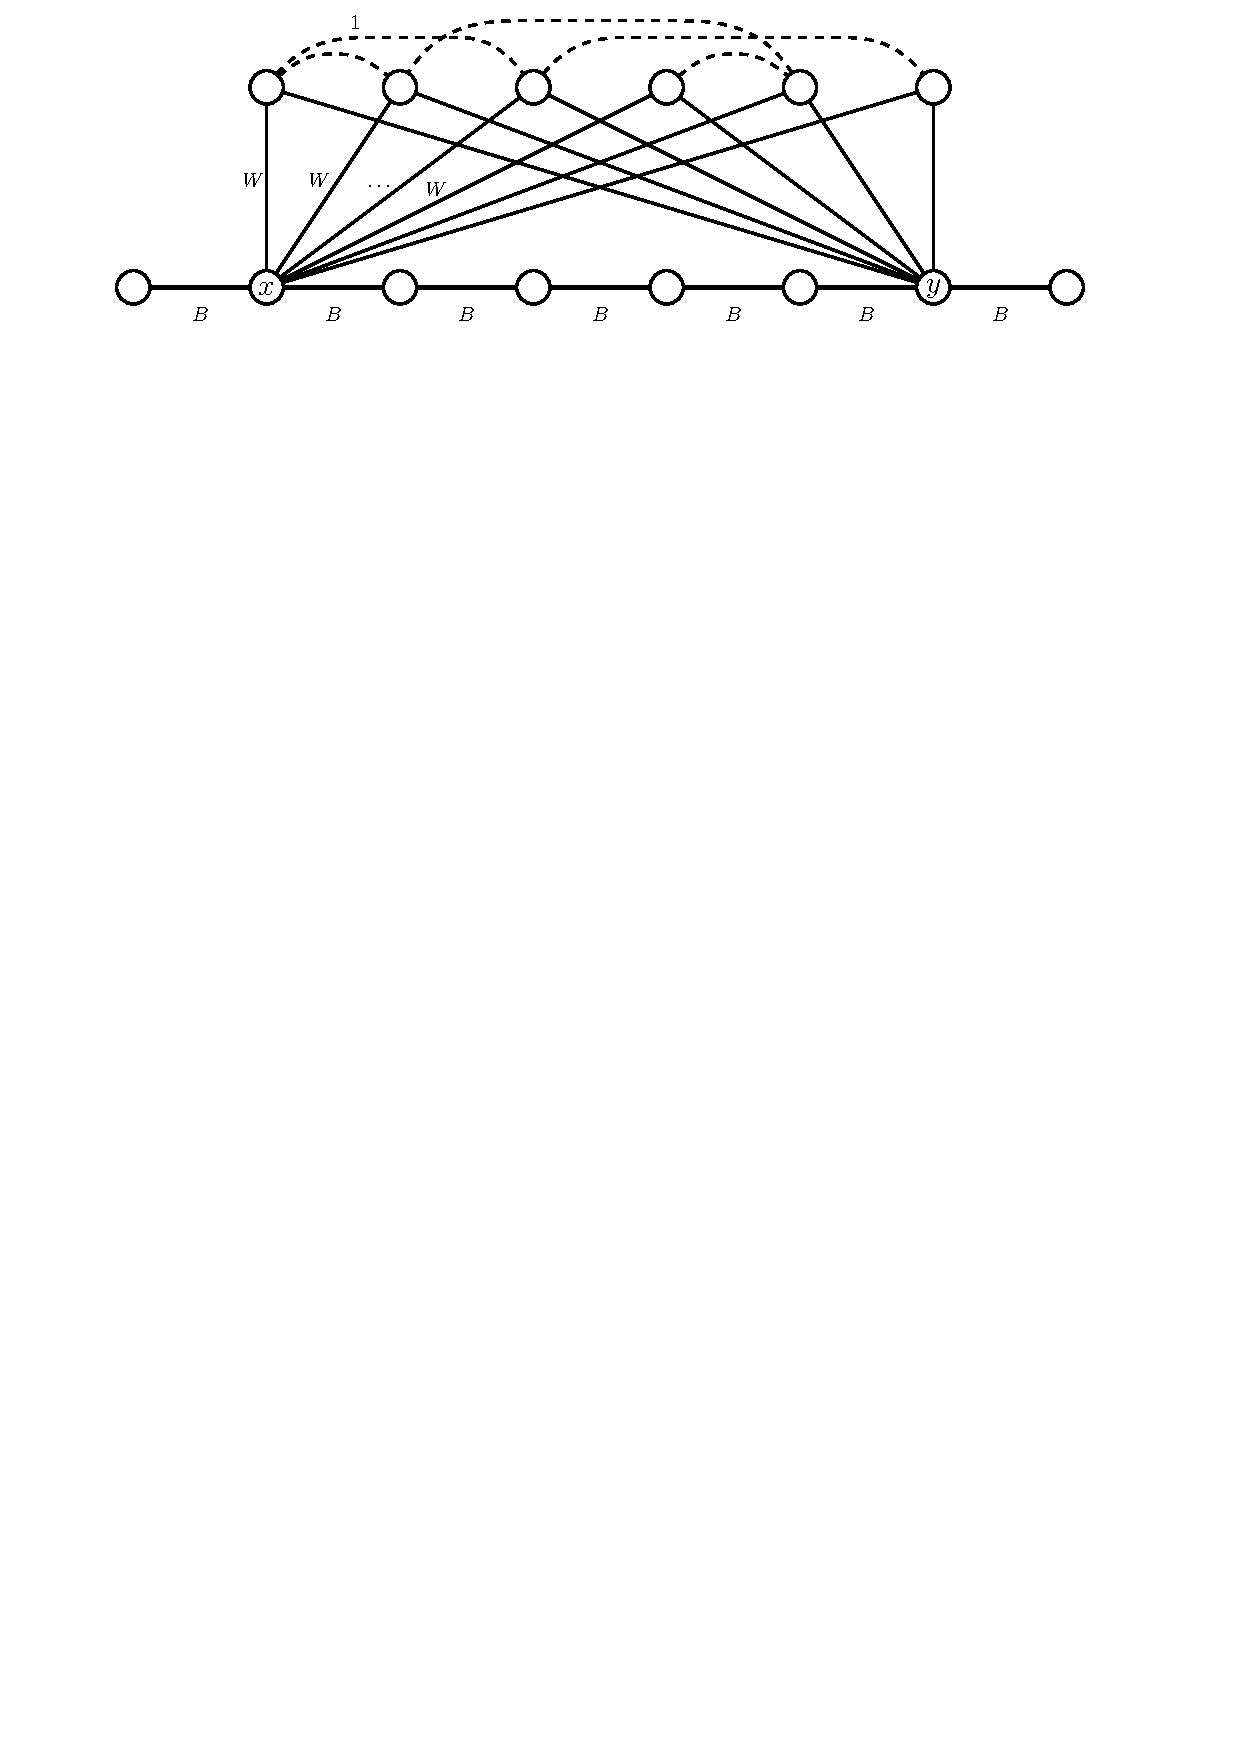
\includegraphics[width=0.3\textwidth]{figs/substitute}
	\caption{Illustration to bounding the cycle length.}
	\label{fig:cascade-illustration}
\end{figure}

\begin{theorem}
	\label{th:cascade-cycles}
	Consider a single merge action of \TAlg.
	There exists an optimal cost reconfiguration with the migration graph, where each cycle have length at most $k$.
\end{theorem}

\begin{proof}
	Assume the contrary, i.e., for each optimal cluster reconfiguration, its migration graph contains a cycle at least $k+1$.
	
	Fix a reconfiguration and its migration graph $G$ that has the shortest length $L$ of the longest cycle, and has the least number of cycles of length $L$.
	Let $p = \lbrace v_1, v_2, \ldots, v_L \rbrace$ be any cycle of length $L$.
	As edge labels are from $\{ 1, 2, \ldots, k \}$, there exists a pair of edges $e, f$ with equal labels.
	
	We show that in such case, we can modify the solution without affecting its cost and feasibility to decrease the number of cycles of length $L$ by $1$.
	This would contradict the assumption that we consider a solution with the minimal number of cycles of length $L$.
	
	We construct a new migration graph $G'$ of equal cost by swapping the (destination) endpoints of $e$ and $f$ (cf. Figure~\ref{fig:cascade-illustration})
	Formally, let $\lbrace a, b \rbrace = e$ and $\lbrace c, d \rbrace = f$.
	We remove $e$ and $f$ and add $e' = \lbrace a, d \rbrace$ and $f' = \lbrace c, d \rbrace$.
	This way we produced a feasible solution.
	
	It remains to show that while decreasing the number of cycles of length $L$, we did not created any new cycles of length at least $L$.
	Assume that adding $e'$ created a new cycle of length at least $L$.
	However, $a$ and $d$ were already connected in $G$ by a directed path of length at least $2$, and a cycle strictly longer than $L$ existed in $G$.
	
	Assume that adding $f'$ created a new cycle $s^*$ of length $L' \geq L$.
	Contrary to the previous case, the directed cycle from $e$ to $b$ might not exist in $G$.
	However, this would mean that $b$ and $e$ were connected by a path of length $L'-1$.
	This means that we might have followed this alternative path from $b$ to $e$ to obtain a cycle strictly longer than $L$ (cf. Figure~\ref{fig:cascade-illustration}).
	
\end{proof}


\begin{theorem}
	Consider a single repartition of DET2.
	The number of clusters it involves is bounded by $k^k$.
	\label{th:cascade}
\end{theorem}

\begin{proof}
	Each node has degree at most $k$.
	Every subset has flow conservation property, hence each cycle traverses one of the nodes of graph origin/core. (no subsets with just incoming edges to the origin part)
	Combine with Theorem \ref{th:cascade-cycles}.
	
\end{proof}


Corollary: Algorithm DET2 is $O(\ell \cdot k \cdot \min \{ \ell, k^k \})$-competitive.
\end{comment}


\section{Improved algorithm for Online Rematching}
\label{sec:k2}



\maciek{Intro: compare to previous 7-competitive algorithm. Note strict competitive ratio vs large additive term. Also, emphasize that in this section the algorithm is different than DET2}

We describe the algorithm \RM for the online rematching problem as follows.
The input to \RM is a sequence of  requests
$\sigma:=\{\sigma_1,\dots, \sigma_m\}, \sigma_t:=\{x,y\} \in V^2, x \neq y$.
We maintain a counter $C_{\set{x,y}}$ for each pair of nodes $\set{x,y}$ and increment it on every remote request between $x$ and $y$.
Once $C_{\set{x,y}} = \lambda$,
reset the counter and collocate the pair arbitrarily in one of the two clusters where $x$ or $y$ resides.

\begin{theorem} \label{thm:k=2}
	The algorithm \RM, for $\lambda=\alpha$, is (strictly) 6-competitive.
\end{theorem}


We charge both \OPT and \RM whenever \RM collocates a pair (i.e., on a collocation event).
%More precisely,we charge them only the cost of the collocation, per such event.
%Hence,we charge the cost of  this collocation to \OPT for the first time.
\RM collocates a pair always with a swap (i.e., two simultaneous migrations),
which  costs $2\alpha$,
while OPT may save some costs by collocating multiple pairs at once, 
 before they inflict too much communication cost.
 Therefore it pays the price of only one migration per pair  (\mahmoud{see Figure \ref{fig:TBD}}).
Hence,
whenever \OPT collocates a pair,
we charge it only the cost of moving a single node to the cluster of the other,
i.e., $\alpha$ (in contrast to $2\alpha$ on \RM).

\textbf{The charging Scheme.}
Consider two  pairs that share a same node, 
i.e.~\emph{intersecting pairs},
and the set of requests that causes the collocation of both pairs,
at some  times during  $[1,m]$.
%i.e.~the entire duration of the sequence.
Observe that \OPT must pay a non-zero cost
for these requests over the entire $\sigma$,
since it cannot have both pairs initially collocated.
%More precisely,
%OPT  pays a total cost at least
%	$\min{ \{ 2\lambda, \lambda+\alpha, 2\alpha \} }$ for, respectively,
%	serving requests to both pairs remotely,
%	serving requests to one pair remotely and collocating the other,
%	or collocating both pairs. 
%
%for serving (some of) these requests remotely or (and) collocating (one of) the pairs,
%regardless of its choices.
%Then the cost per pair, in particular the cost w.r.t.~$\{u,v\}$, is
%$\mathit{OPT} (\sigma_{\{u,v\}}) \geq c_{R_t} / 2$.
%
However,
we can charge the whole cost to \OPT only the first time \RM collocates a pair,
and not at any consequent time when \RM collocates it a second time.
Otherwise,
 \OPT is possibly charged for a same cost repeatedly.
For this reason,
we charge \OPT a cost inflicted by a pair,
if and only if  \OPT incurs the cost some time since the last time \RM separated the pair.
%%

\begin{proof}[Proof of Theorem \ref{thm:k=2}]
	Assume on request $\sigma_{t}=\set{u,v}$, 
	i.e., at (time) $t$,
	Alg collocates the pair $\set{u,v}$.
	This means,
	the value of $C_{\set{u,v}}$ at $t$,
	denoted by $C^t_{\set{u,v}}$, 
	reaches $\lambda$ immediately before \RM resets the counter.
	I.e.,
	$ C^t_{\set{u,v}} = \lambda$.
	%	In case the first collocation of $\set{u,v}$ occurs at $t$,
	%	if the pair is collocated in the initial configuration then
	%	we set $t''=0$,
	%	else,
	%	we set $ t'' = -\infty, t'=0$.
	We denote the set of all requests to a pair $\set{x,y}$ that arrive
	during $[t_1,t_2]$ by $\sigma_{\set{x,y}}[t_1,t_2]$,
	and its overall cost to \OPT by
	$\mathit{OPT} (\sigma_{\{u,v\}}[t_1,t_2])$.
	We may use $\sigma_{\set{x,y}}$ whenever
	 the interval $[t_1,t_2]$ is clear from the context.
	%
	%Else, this is not the first time and
	%Alg collocates $\{u,v\}$ also some time prior to $t$.
	
	If $t$ is not the first time that \RM collocates $\{u,v\}$ then
	let $0 < t' < t$ be the latest time when \RM separates $\set{u,v}$
	in order to collocate some intersecting pair
	$\{x,y\} \neq \{u,v\}, \{x,y\} \cap \{u,v\} \neq \emptyset$, 
	e.g.,
	$\{x,y\}=\{u,w\}$.
	Else,
	$t$ is the first time that \RM collocates $\{u,v\}$ and let $t' := 0$.
	Similarly,
	if $t' > 0$ is not the first time that \RM  collocates $\{u,w\}$ 
	then let $0 < t'' < t'$ be the latest time before $t'$ when \RM separates $\set{u,w}$.
	Else,
	$t'$ is the first time that \RM collocates $\{u,w\}$ and we let $t''=0$.
	%
	
	First,
	we bound  costs incurred by \RM for requests that
	lead to the collocation of $\{u,v\}$ at time $t \in T$, where
	$T := \{ i \in [1,m] ~\vert~ \exists \{x,y\}: C^{i}_{\{x,y\}} = \lambda \}$
	is the set of times when \RM performs a collocation.
	By definitions of $t$ and $t'$,
	the overall cost of requests in $\sigma_{\set{u,v}}$ incurred by \RM,
	i.e., the total cost of remote serving
	and the moving cost, is
	$\lambda + 2\alpha$.	
	Next,
	we bound costs incurred by \RM
	for requests that do not lead to collocations until the  end of the sequence at $t=m$.
	Assume $\{u,v\}$ is not collocated at $t=m$
	and $0 < C^{m}_{ \{u,v\} } < \lambda $,
	which means \RM pays $C^{m}_{ \{u,v\} }$
	for  requests in $\sigma_{\set{u,v}}(t',m]$.
    Then the overall cost to \RM is
$	\mathit{RM} (\sigma)
=
\sum_{ t \in T}(\lambda + 2\alpha) +
\sum_{\{u,v\}} C^{m}_{\{u,v\}}	
$.
%	\begin{align*}	%\label{eq:costAlg}
%	\mathit{RM} (\sigma)
%	=
%	\sum_{ t \in T}(\lambda + 2\alpha) +
%	\sum_{\{u,v\}} C^{m}_{\{u,v\}}	
%	\leq
%	\sum_{ t \in T}(\lambda + 2\alpha) +
%	\sum_{\{u,v\}} C^{m}_{\{u,v\}}	
%	=
%	\sum_{ t \in T} 3\alpha +
%	\sum_{\{u,v\}} C^{m}_{\{u,v\}}
%	.
%	\end{align*}
	
	Next,
	we bound  costs incurred by \OPT for requests that trigger collocation of $\{u,v\}$ at $t \in T$.
	If $t$ is the first time that \RM collocates $\{u,v\}$ then  \OPT pays
	$\lambda$ for serving requests in $\sigma_{\set{u,v}}[0,t]$ (remotely),
	or $\alpha$ for collocating the pair and
	serving (some of) the requests with  cost zero.
	Therefore in this case,
	$\OPTM (\sigma_{\{u,v\}}(0,t]) \geq  \min{\{ \lambda,\alpha \}}$.
	%
	Otherwise,
	it is not the first collocation and
	consider times $t'$ and $t''$ as define previously,
	 and let 
	$R_t := \sigma_{\{u,w\}}(t'',t'] \cup \sigma_{\{u,v\}}(t',t] $.
	We define $R_{t'}$ for the collocation at $t'$  analogously.
	Then,
	$\OPTM(R_t) = \mathit{OPT} (\sigma_{\{u,w\}}) 
	+ \OPTM(\sigma_{\{u,v\}}) $.
	Note that \OPT cannot have both pairs collocated at the same time.
	However, it can have one of the pairs already collocated prior to its respective interval.
	Let us assume  \OPT has one pair,
	e.g.~$\{u,v\}$ collocated already prior its respective interval, i.e.~$(t',t]$,
	 and keeps it so during the interval.
	 Then it pays zero while serving $\sigma_{\{u,v\}}$.
	Hence,
	it must pay $\alpha$ for collocating the other pair, in this case $\{u,w\}$,
	or (resp., and) it pays (resp., up to) $\lambda$ for serving (resp., some of) requests in $\sigma_{\{u,w\}}$. 
	Therefore in any case $\OPTM(R_t) \geq  \min{\{ \lambda,\alpha \}}$.
	\begin{comment}
	We distinguish three (non-exhaustive) cases for the cost to \OPT w.r.t.~$R_t$.
	Latter,
	 we argue that \OPT cannot save cost by deviating from these cases.
	\begin{enumerate}[label=\roman*.]
		\item
		\OPT collocates $\{u,w\}$ at  $t''$, $\{u,v\}$  at $t'$,
		and keeps them so during $(t'',t']$ and $(t',t]$, respectively.
		Therefore it serves all requests in $R_t$ with no additional cost and
		let $\OPTM_1 (R_t) := 2\alpha$.
		\item
		\OPT has one of the pairs  already collocated and the other pair separated,
			  prior to and during their respective intervals.
		Hence,
		it pays only $\lambda$ for serving all requests in $R_t$
		and let $\OPTM_2 (R_t) := \lambda$.
		\item
		\OPT has one of the pairs already collocated prior to its interval,
		and it collocates the other pair during the respective interval.
		Then it pays 0 for one pair and $\alpha$ for the other and 
		let $\OPTM_3 (R_t) := \alpha$.
	\end{enumerate}
%	We consider cases (ii) and (iii) also for the pair $\{u,w\}$, symmetrically.
	If \OPT behaves in one of these cases,
	then
	$\mathit{OPT} (R_t) \geq
		\min{\{ \OPTM_1(R_t), \OPTM_2(R_t), \OPTM_3(R_t) \}}  =
		\min{ \{ \lambda, \alpha \}}$.
	Otherwise,
	\OPT deviates from these cases,
	e.g.~by collocating a pair after paying for some of requests to this pair.
	However,
	no deviation can decrease the cost to \OPT. \mahmoud{prove this!}
	Therefore in any case,
	$\mathit{OPT} (R_t) \geq  \min{ \{ \lambda, \alpha \}}$.
	\end{comment}
	
	It remains to bound the cost  incurred by \OPT due to requests to $\{u,v\}$ that do not lead to its collocation until the end of the sequence at $t=m$.
	We bound the cost analogously to the case where \RM collocates $\{u,v\}$.
	If $\{u,v\}$ is not collocated in the initial matching
	and \RM never collocates it,
	then $ C^{m}_{ \{u,v\} } =| \sigma_{\{u,v\}}[1,m] |$.
	\OPT pays
	$\mathit{OPT} (\sigma_{\{u,v\}}[1,m]) 
	\geq \min{ \{ \alpha, C^{m}_{ \{u,v\} } \} }$,
	for collocating this pair or (and) paying for (resp.~some of) requests in $\sigma_{\{u,v\}}[1,m]$.
	Else,
	either $\{u,v\}$ is collocated in the initial matching
	or \RM collocates it at some point.
	Then there exists an intersecting pair $\set{u,w}$
	that is collocated by \RM at $t' < m$ (separating $\{u,v\}$).
	We define times $t'' < t' < m$ similarly as in the former case.
	Let $R^*_{\{u,v\}} := \sigma_{\{u,w\}} (t'',t'] \cup \sigma_{\{u,v\}} (t',m]$.
	Then,
	\OPT must pay for collocating at least one pair or (and) serving requests 
	to the other pair remotely.
	Thus,
	$\mathit{OPT} (R^*_{\{u,v\}}) 
	\geq  \min{ \{ C^{m}_{ \{u,v\}}, \alpha \}}$.
	
	Next, we sum up all costs incurred by \OPT.
	By definitions of $R_t$ and $R^*_{\{u,v\}}$, we have either
	$R_{t'} \cap R_t = \sigma_{\{u,w\}}$ or
	$R_{t'} \cap R^*_{\{u,v\}} = \sigma_{\{u,w\}}$
	(\mahmoud{See figure \ref{fig:doubleCount}}). 
	This means,
	$\OPTM ( \sigma_{\{u,w\}})$
	is counted at most twice in each of  the expressions
	$\mathit{OPT} (R_{t'}) + \mathit{OPT} (R_t)$
	and  
	$\mathit{OPT} (R_{t'}) + \mathit{OPT} (R^*_{\{u,v\}})$.
	Hence,
	for all collocations performed by \RM,
	and for final costs at $t=m$,
	\OPT pays at least 
	$\frac{1}{2}(
	\sum_{ t \in T } \mathit{OPT} (R_t) +
	\sum_{\{u,v\}} \mathit{OPT} (R^*_{\{u,v\}})
	) $.
	Then,
	the total cost to \OPT is
	
	\begin{align*} 	%\label{eq:costOPT}
		\mathit{OPT} (\sigma)
		&=
		\frac{1}{2}
		\Big(
		\sum_{ t \in T} \mathit{OPT} (R_t) 
		+ \sum_{\{u,v\}}\mathit{OPT} (R^*_{\{u,v\}})
		\Big)	\\
		&\geq
		\Big(
		\sum_{ t \in T} \min{ \{ \lambda, \alpha \}}  +
		\sum_{\{u,v\}} \min{ \{C^{m}_{\{u,v\}} , \alpha \} } 
		\Big)		
		=
		\frac{1}{2}		
		\Big(
		\sum_{ t \in T} \alpha  
		+ \sum_{\{u,v\}} C^{m}_{\{u,v\}}
		\Big).
	\end{align*}

Finally, we have

\begin{align*}
	\mathit{ALG} (\sigma)	/
	\mathit{OPT} (\sigma)
	\leq
	2\Big(
	\sum_{ t \in T} 3\alpha +
	\sum_{\{u,v\}} C^{m}_{\{u,v\}}
	\Big)	 \big /
	\Big(
	\sum_{ t \in T} \alpha  
	+ \sum_{\{u,v\}} C^{m}_{\{u,v\}}  
	\Big)	< 6.
\end{align*}
%	The claim follows from here.

\end{proof}

Major:

\maciek{I feel slightly uneasy here: "In particular,
we charge \OPT a cost incurred by requests in
$\sigma_{\{u,w\}}$ and $\sigma_{\{u,v\}}$,
if and only if  \OPT incurs the cost within  intervals $(t'', t']$ and $(t', t]$,
respectively.
\mahmoud{this is only for intuition but a key statement. It is meant to say: \OPT may pay cost for the same two pairs outside the intervals. But we don't charge \OPT  those costs at $t$. This way we avoid over charging \OPT as only intervals $r_{t'}$ and $r_t$ can overlap which leads to double charging and we take care of it.}
"}

\maciek{"Observe that for requests in $R_t$". First the separate sentence with the definition of $R_t$ (it is challenging enough to just understand it. Then reason why it pays the minimum of three values (I don't see it, and later you show that cost(rt) is at least minimum of other two values). Is it a consequence of three cases? \mahmoud{the duration is the key and the latter duration is different. I reworded the whole thing. And yes, the same three cases can be used to explain this observation. Now the "some of" in the parenthesis might be enough for a clue. This observation is  used implicitly in the proof when it bounds the cost of first time collocation.}}

\maciek{"We charge \OPT the cost
$\mathit{\OPT} (\sigma_{\{u,v\}}[1,t]) 
\geq \min{ \{ \alpha, C^{m}_{ \{u,v\} } \} }$,
for collocating this pair or (and) paying (partially) for requests in $\sigma_{\{u,v\}}[1,t]$." No issues with charge sharing from "regular collocation" case? Maybe I just don't understand "partially" here. Not necessarily rewrite! Just maybe check if it's true.
\mahmoud{this is the cost of first collocation of $\{u,v\}$. "partially" is confusing and now it says "some of" instead.}}

Minor:

\maciek{The big inequality is impressive, but not a lot change in each row. Instead, bound the cost of ALG separately in one line, and the cost of \OPT in another. (possibly far away from eachother) \mahmoud{done}}

\maciek{Remove all "charge both". Just sum up costs. I would say not use "charge" at all, but it's up to you. \mahmoud{done}}


\maciek{Structure in paragraphs. 3 parts: first collocation, regular collocation and unfinished. Do this for ALG and then for \OPT, and do not mix (unless I don't see some dependencies). Start each paragraph by the sentence that says what the paragraph is about (first/opt, regular/alg etc.). Assume that the reader reads only the first sentence of each paragraph (if it's short), and the proof structure must be clear from this. Some other important things go to their own paragraph too, and the first sentence must describe what we do there.}

\maciek{$R_t$ is the central concept in this proof. Possibly even start with the paragraph: charging \OPT, regular collocation. Make this definition in its separate line to further emphasize? It would suffice for a profesional to see the definiton of $t''/t'$ and this line to convince himself that the proof is correct.}

\maciek{I think that "deviate" is OK to use like this.}

Notation:

\maciek{End of the time proposition: $t_e / t^* / T$ instead of $m$? Or capital $T$ (but I am aware of the conflict)}

\maciek{Instead of $cost_{opt}$ just use opt / alg?}

\maciek{Consider naming the adjacent edges $e$ and $f$.}

\section{Distributed implementation.}
The algorithm PPL from Section~\ref{sec:ppl} can be distributed
similarly to the approach in~\cite{sigmetrics19_partitioning}.
The algorithm for $k=2$ from Section~\ref{sec:k2} performs only local communication for each request: counters are kept on the clusters and updated locally, and each migration concerns only two clusters.
\medskip

In the rest of this section, we propose the distributed implementation of the algorithm for $k=3$ from Section~\ref{sec:k3}.
The algorithm performs two non-local operations:
\begin{enumerate}
	\item Broadcasting the end of the phase.\label{it:broadcast}
	\item Component merge.
	\label{it:merge}
\end{enumerate}

If a component reaches size $4$ or fresh cluster is not found, we conclude that no perfect partition exists.
Then, we end the phase and broadcast (\maciek{TODO: efficient broadcast cite}) the message to  reset the counters in all clusters.

A merge of two components may require finding a third cluster that contains $3$ alone nodes (for details see the proof of Lemma~\ref{lem:1req})).
We say that a cluster containing $3$ alone nodes is \emph{fresh}.
In the following, we show how to efficiently find a fresh cluster in a distributed manner.
We organize the clusters into an arbitrary rooted balanced binary tree (\maciek{TODO: how to do it efficiently? Does not matter much, as this is performed once at the beginning}), and we broadcast the root to each cluster.
Each cluster maintains the counter of fresh clusters in its subtree.
To find a fresh cluster, we traverse an arbitrary path of non-zero counters from the root.
Upon encountering a fresh cluster, we stop the traversal and decrease the counters on the followed path by $1$.

The operation (\ref{it:broadcast}) requires a single broadcast, and the operation (\ref{it:merge}) requires $O(\log(\ell))$ communication.
Each of these may occur, on average, every $\alpha$ external requests.


\bibliographystyle{ACM-Reference-Format}
\bibliography{references}  

\appendix


\section{Omitted results (for our future papers)}

\begin{enumerate}
	\item Costly cascade example (it is easy to present $k^2$ and $k\cdot \sqrt{k}$ (with different approach), and then we can combine these to obtain $k^3$)
	
	\item $k$-competitive algorithm for the ring communication pattern
	
	\item lower and upper bound $k+1$ for two clusters, perfect partition and the optimal configuration reachable within one swap
	
	\item The lower bound $(k \cdot \ell - k - \ell) / 2$ can be easily improved to $(k \cdot \ell - k - 1) / 2$ by playing a simple caching game in the first cluster, instead of just giving away the $k-1$ "blocker" (the caching game would build it gradually)
	
\end{enumerate}


\end{document}
